

\chapter{Procedures for system assembly/installation/testing/commisioning} \label{CHAPTERASSEMBLY}

\section{System assembly}
\subsection{Cable construction}
\subsubsection{Construction of ACT/E - Cable for motor encoder} \label{CONSTRUCTION:ACTE}
The encoder cable is supplied together with the motor combination (see section~\ref{DEVICE:COMBINATION1}). Instead of purchasing for 4.2 meters of cable for encoder, a better option is ordering 60cm for each ordered motor combination. One cable side comes already attached to the motor combination. However, the other side requires a 10-pin female connector for flat cable (section~\ref{DEVICE:10pinF(Encoder)}). Please follow these procedures and use figure~\ref{FIG:ACTEconstruction} as a reference:
\begin{itemize}
  \item (1) See that this encoder cable already comes with the motor combination. As mentioned in section~\ref{CABLETYPE:Electric(Encoder)}, order a 60cm length.
  \item (2) Leave a piece of cable/wire envelops striped at each cable end.
  \item (3) Install the 10pinF(Encoder) connector at the free cable side. Use the section~\ref{DEVICE:10pinF(Encoder)} as a reference for pinout. Use the procedures described at subsection~\ref{CRIMPING10pin} for the connector installation.
\end{itemize}
\begin{figure}
  \centering
  % Requires \usepackage{graphicx}
  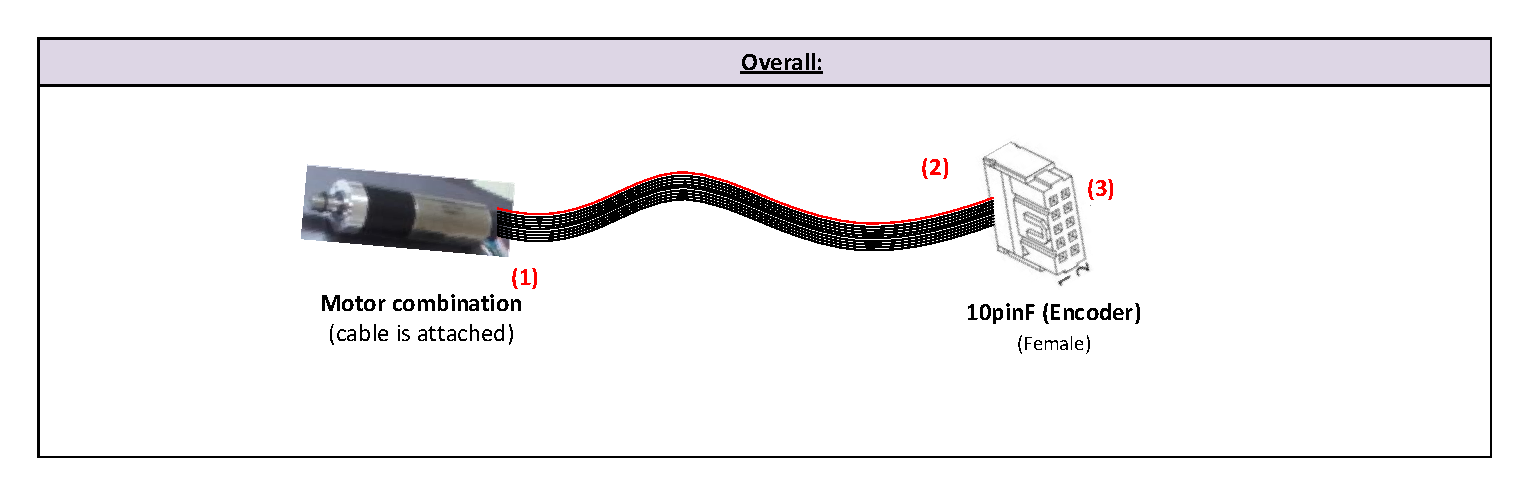
\includegraphics[angle=90,width=1\columnwidth]{figs/body03/FIGACTEconstruction.pdf}\\
  \caption[Construction of ACT/E - Cable for motor encoder]{Construction of ACT/E - Cable for motor encoder}
  \label{FIG:ACTEconstruction}
\end{figure}
\subsubsection{Construction of ACT/H - Cable for motor Hall effect sensor} \label{CONSTRUCTION:ACTH}
The Hall sensor cable is composed by 5 free wires, and it is supplied together with the motor combination (see section~\ref{DEVICE:COMBINATION1}). Instead of purchasing for 4.2 meters of cable for hall sensor, a better option is ordering 60cm for each ordered motor combination. One cable side comes already attached to the motor combination. However, the other side requires a Molex Micro-Fit connector (section~\ref{DEVICE:microHall}). Please follow these procedures and use figure~\ref{FIG:ACTHconstruction} as a reference:
\begin{itemize}
  \item (1) See that this hall sensor cable already comes with the motor combination. As mentioned in section~\ref{CABLETYPE:Electric(Hall)}, order a 60cm length.
  \item (2) Leave a piece of each wire envelop striped at the free end.
  \item (3) Install the Micro-Fit connector at the free wire ends. Use the section~\ref{DEVICE:microHall} as a reference for pinout. Use the procedures described at subsection~\ref{CRIMPINGmicro} for the connector installation.
\end{itemize}
\begin{figure}
  \centering
  % Requires \usepackage{graphicx}
  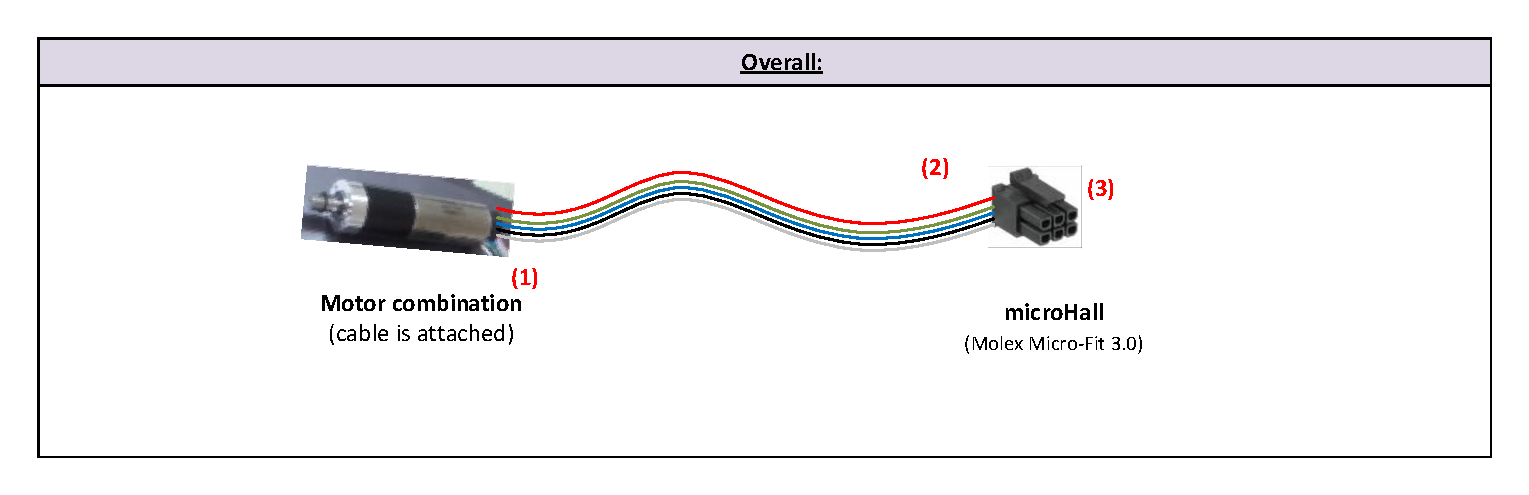
\includegraphics[angle=90,width=1\columnwidth]{figs/body03/FIGACTHconstruction.pdf}\\
  \caption[Construction of ACT/H - Cable for motor Hall effect sensor]{Construction of ACT/H - Cable for motor Hall effect sensor}
  \label{FIG:ACTHconstruction}
\end{figure}

\subsubsection{Construction of ACT/M - Cable for motor supply} \label{CONSTRUCTION:ACTM}
The motor cable is composed by 3 free wires, and it is supplied together with the motor combination (see section~\ref{DEVICE:COMBINATION1}). Instead of purchasing for 4.2 meters of cable for motor supply, a better option is ordering 60cm for each ordered motor combination. One cable side comes already attached to the motor combination. However, the other side requires a Molex Mini-Fit connector (section~\ref{DEVICE:miniMotor}). Please follow these procedures and use figure~\ref{FIG:ACTMconstruction} as a reference:
\begin{itemize}
  \item (1) See that this motor cable already comes with the motor combination. As mentioned in section~\ref{CABLETYPE:Electric(Motor)}, order a 60cm length.
  \item (2) Leave a piece of each wire envelop striped at the free end.
  \item (3) Install the Mini-Fit connector at the free wire ends. Use the section~\ref{DEVICE:miniMotor} as a reference for pinout. Use the procedures described at subsection~\ref{CRIMPINGmicro} for the connector installation.
\end{itemize}
\begin{figure}
  \centering
  % Requires \usepackage{graphicx}
  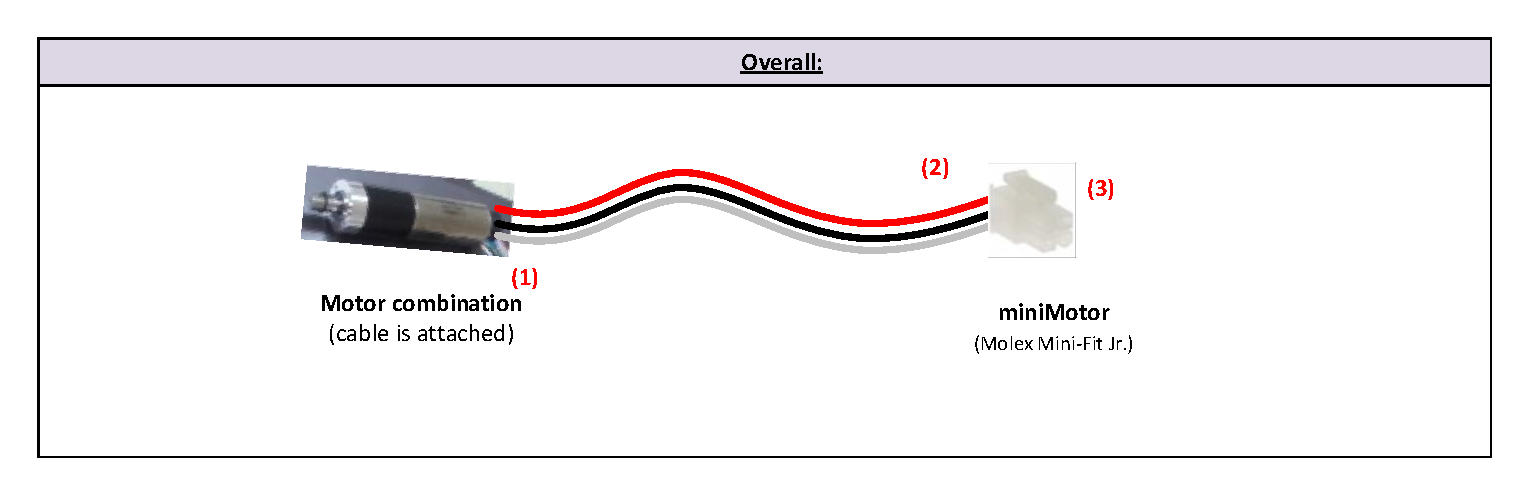
\includegraphics[angle=90,width=1\columnwidth]{figs/body03/FIGACTMconstruction.pdf}\\
  \caption[Construction of ACT/M - Cable for motor supply]{Construction of ACT/M - Cable for motor supply}
  \label{FIG:ACTMconstruction}
\end{figure}

\subsubsection{Construction of CAN/D-D - Cable for CAN between drivers} \label{CONSTRUCTION:CANDD}
Use figure~\ref{FIG:CANDDconstruction} as a reference for the correct construction of this cable type. Please follow these procedures:
\begin{itemize}
  \item (1) Cut a piece of the CAN cable (described in section~\ref{CABLETYPE:CAN}) to the correct length indicated in the cable list (figure~\ref{FIG:CABLELIST}).
  \item (2) Leave a piece of cable/wire envelops striped at each cable end.
  \item (3) If an Ethernet cable is used: a) use a pair as CAN-High and CAN-Low; b) use a wire from another pair as the CAN GND; c) ignore the other wires.
  \item (4) Install the connector microCAN - Molex Micro-Fit 3.0 in both cable sides. Use the section~\ref{DEVICE:microCAN} as a reference for pinout. Installation steps:
  \begin{itemize}
    \item a) Use the procedures described at subsection~\ref{CRIMPINGmicro} for the connector installation.
    \item b) Please note: the cable shield must be connected at only one cable side (pin 4)!
    \item c) At the other side, please cut off the shield near the Molex connector or just do not plug it!
  \end{itemize}
\end{itemize}
\begin{figure}
  \centering
  % Requires \usepackage{graphicx}
  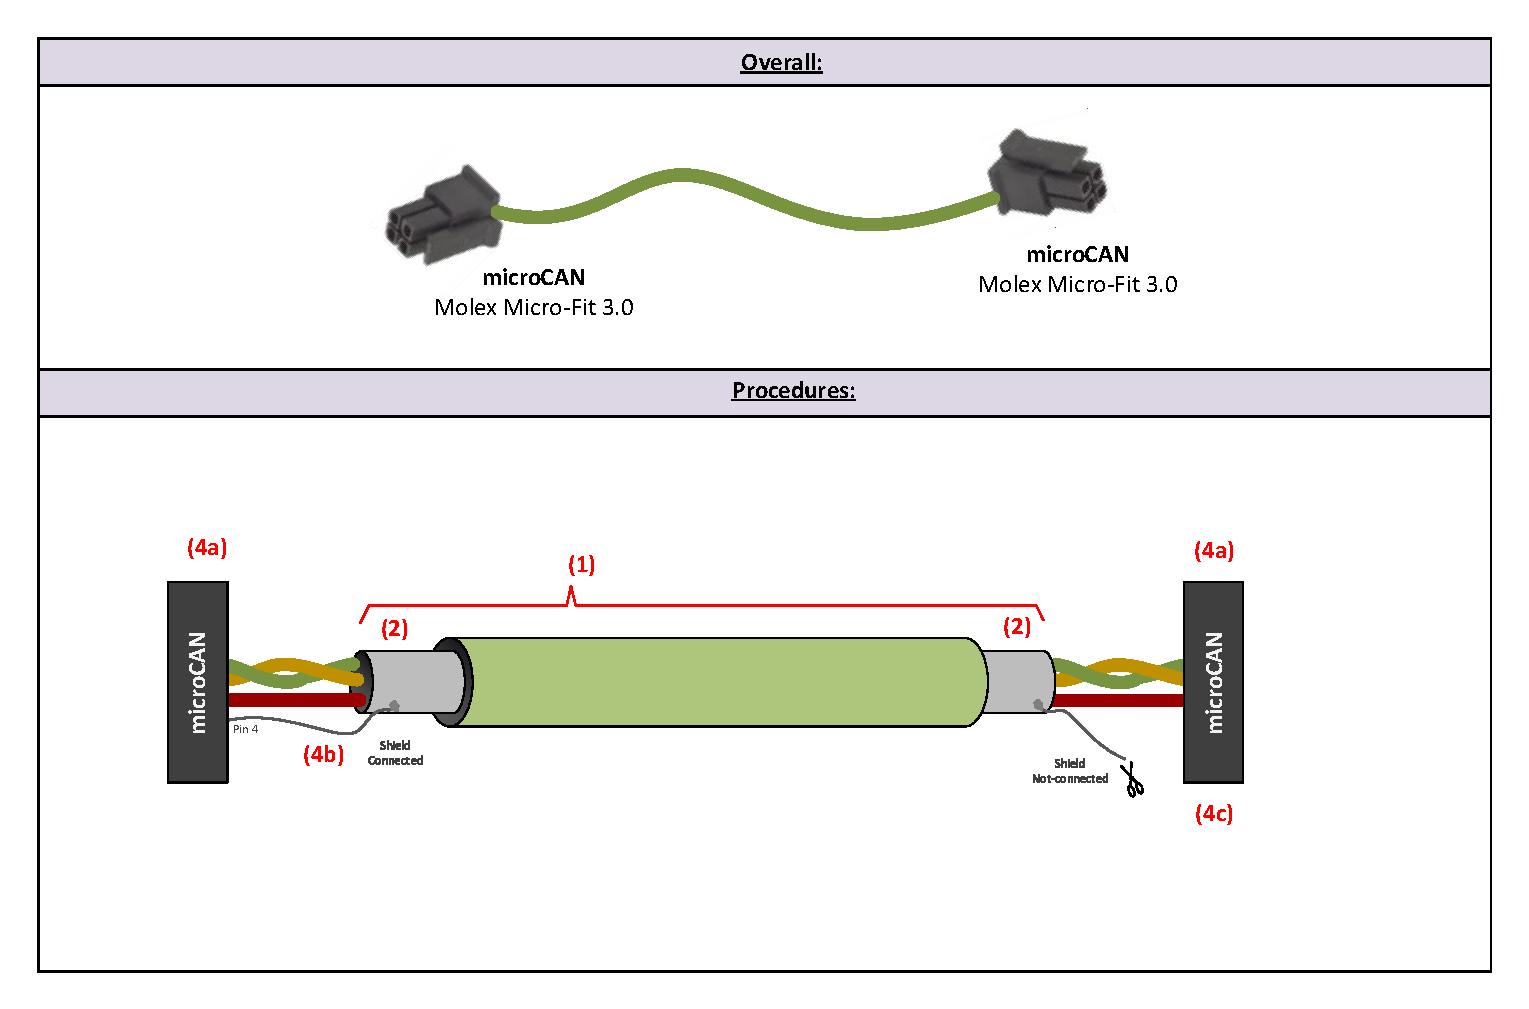
\includegraphics[angle=90,width=1\columnwidth]{figs/body03/FIGCANDDconstruction.pdf}\\
  \caption[Construction of CAN/D-D - Cable for CAN between drivers]{Construction of CAN/D-D - Cable for CAN between drivers}
  \label{FIG:CANDDconstruction}
\end{figure}

\subsubsection{Construction of CAN/I-Dc - Cable for CAN between driver and an interface (shield cut)} \label{CONSTRUCTION:CANIDc}
Use figure~\ref{FIG:CANIDcconstruction} as a reference for the correct construction of this cable type. Please follow these procedures:
\begin{itemize}
  \item (1) Cut a piece of the CAN cable (described in section~\ref{CABLETYPE:CAN}) to the correct length indicated in the cable list (figure~\ref{FIG:CABLELIST}).
  \item (2) Leave a piece of cable/wire envelops striped at each cable end.
  \item (3) If an Ethernet cable is used: a) use a pair as CAN-High and CAN-Low; b) use a wire from another pair as the CAN GND; c) ignore the other wires.
  \item (4) Install the connector DB9F(SH) - Shielded DB9 (Female) at this cable side. Use the section~\ref{DEVICE:DB9F(SH)} as a reference for pinout. Installation steps:
  \begin{itemize}
    \item a) Use the procedures described at subsection~\ref{CRIMPINGDB9} for the connector installation.
    \item b) Please note: the cable shield must be connected to this DB9 (pin 5).
  \end{itemize}
  \item (5) Install the connector microCAN - Molex Micro-Fit 3.0 at this cable side. Use the section~\ref{DEVICE:microCAN} as a reference for pinout. Installation steps:
  \begin{itemize}
    \item a) Use the procedures described at subsection~\ref{CRIMPINGmicro} for the connector installation.
    \item b) Please note: the cable shield must be cut off near this Molex connector. Do not plug the shield envelopment at this side!
  \end{itemize}
\end{itemize}
\begin{figure}
  \centering
  % Requires \usepackage{graphicx}
  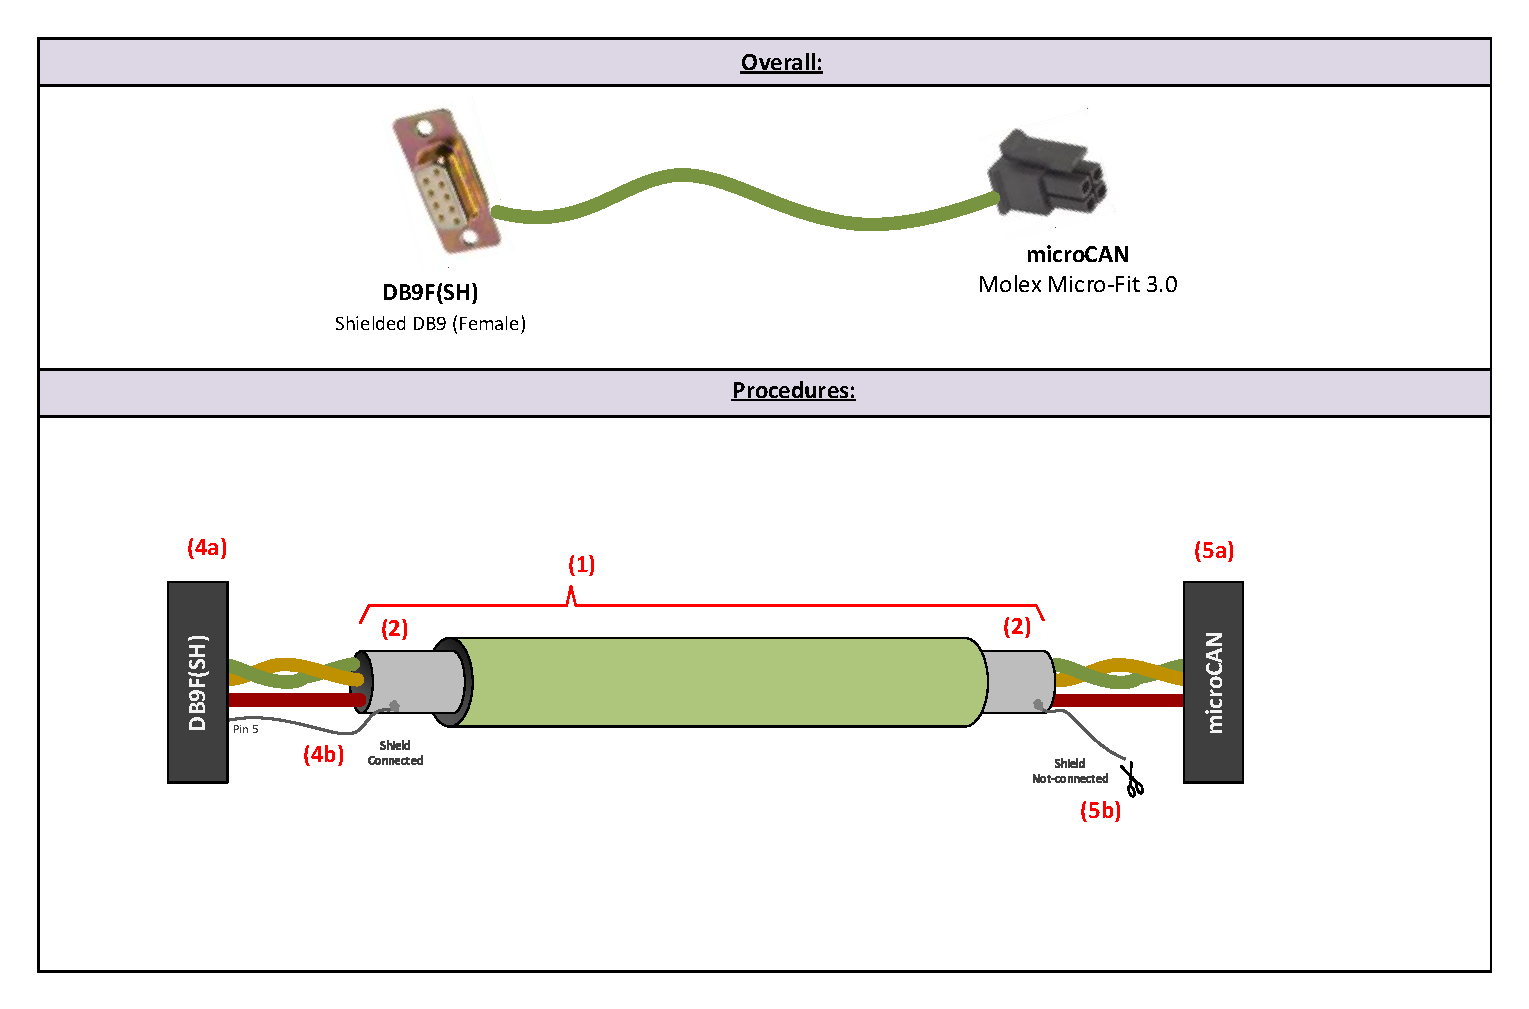
\includegraphics[angle=90,width=1\columnwidth]{figs/body03/FIGCANIDcconstruction.pdf}\\
  \caption[Construction of CAN/I-Dc - Cable for CAN between driver and an interface (shield cut)]{Construction of CAN/I-Dc - Cable for CAN between driver and an interface (shield cut)}
  \label{FIG:CANIDcconstruction}
\end{figure}

\subsubsection{Construction of CAN/I-Dp - Cable for CAN between driver and an interface (shield pass)} \label{CONSTRUCTION:CANIDp}
Use figure~\ref{FIG:CANIDpconstruction} as a reference for the correct construction of this cable type. Please follow these procedures:
\begin{itemize}
  \item (1) Cut a piece of the CAN cable (described in section~\ref{CABLETYPE:CAN}) to the correct length indicated in the cable list (figure~\ref{FIG:CABLELIST}).
  \item (2) Leave a piece of cable/wire envelops striped at each cable end.
  \item (3) If an Ethernet cable is used: a) use a pair as CAN-High and CAN-Low; b) use a wire from another pair as the CAN GND; c) ignore the other wires.
  \item (4) Install the connector DB9F(SH) - Shielded DB9 (Female) at this cable side. Use the section~\ref{DEVICE:DB9F(SH)} as a reference for pinout. Installation steps:
  \begin{itemize}
    \item a) Use the procedures described at subsection~\ref{CRIMPINGDB9} for the connector installation.
    \item b) Please note: the cable shield must be connected to this DB9 (pin 5).
  \end{itemize}
  \item (5) Install the connector microCAN - Molex Micro-Fit 3.0 at this cable side. Use the section~\ref{DEVICE:microCAN} as a reference for pinout. Installation steps:
  \begin{itemize}
    \item a) Use the procedures described at subsection~\ref{CRIMPINGmicro} for the connector installation.
    \item b) Please note: the cable shield must be connected at this Molex connector (pin 4)!
  \end{itemize}
\end{itemize}
\begin{figure}
  \centering
  % Requires \usepackage{graphicx}
  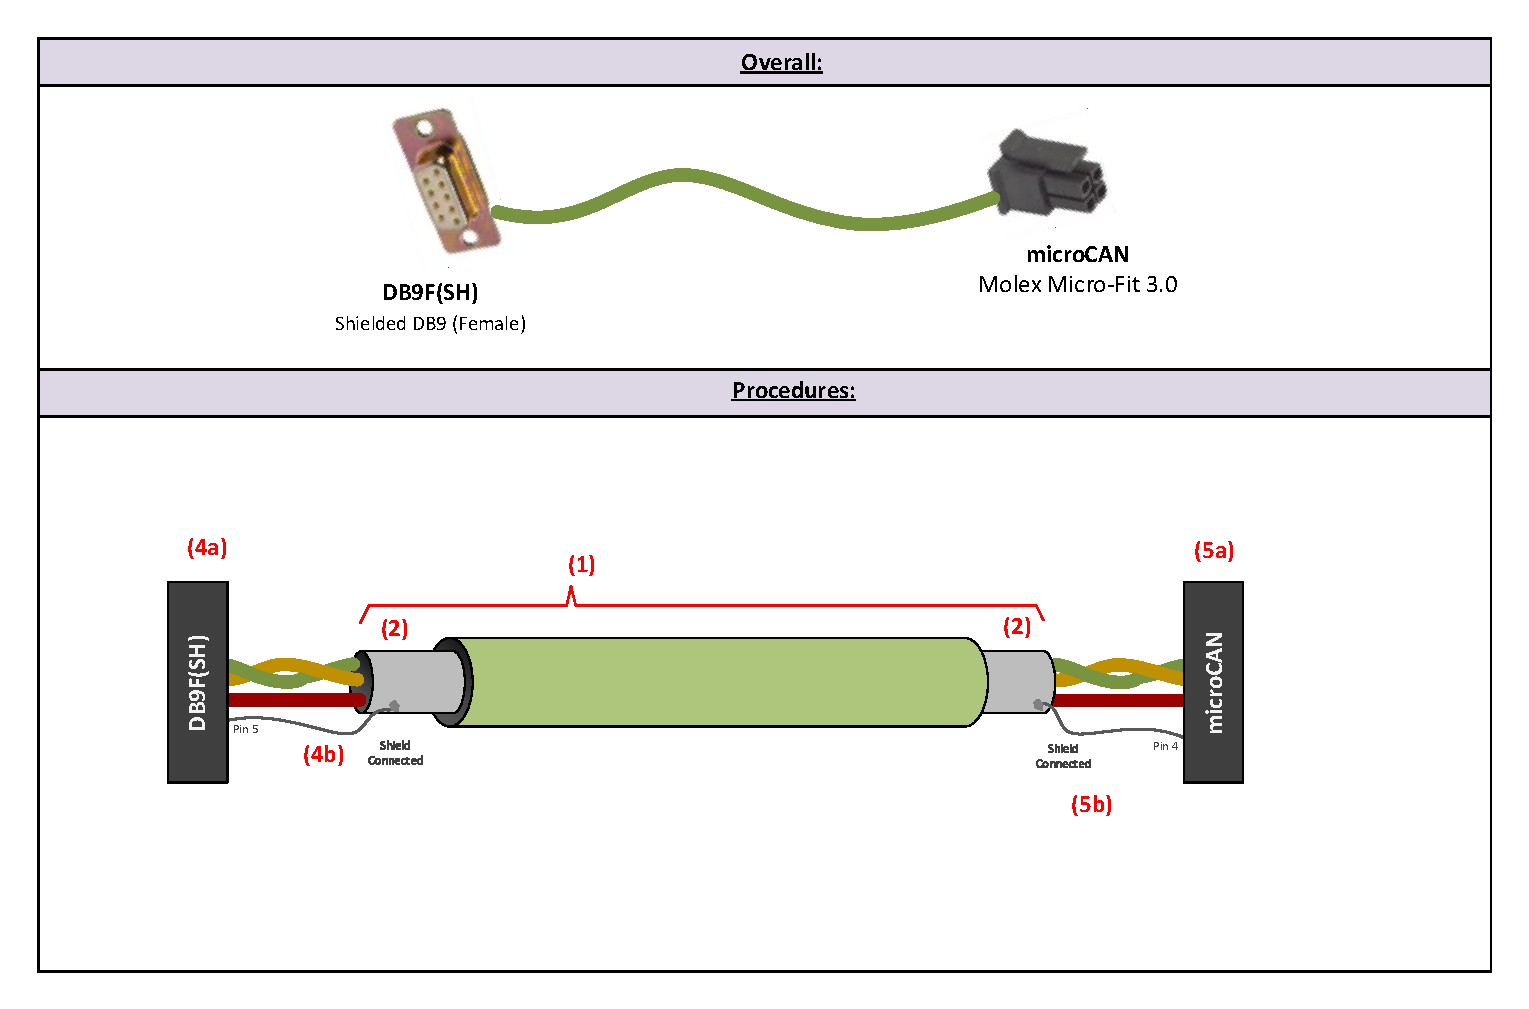
\includegraphics[angle=90,width=1\columnwidth]{figs/body03/FIGCANIDpconstruction.pdf}\\
  \caption[Construction of CAN/I-Dp - Cable for CAN between driver and an interface (shield pass)]{Construction of CAN/I-Dp - Cable for CAN between driver and an interface (shield pass)}
  \label{FIG:CANIDpconstruction}
\end{figure}

\subsubsection{Construction of CAN/I-I - Cable for CAN between interfaces} \label{CONSTRUCTION:CANII}
Use figure~\ref{FIG:CANIIconstruction} as a reference for the correct construction of this cable type. Please follow these procedures:
\begin{itemize}
  \item (1) Cut a piece of the CAN cable (described in section~\ref{CABLETYPE:CAN}) to the correct length indicated in the cable list (figure~\ref{FIG:CABLELIST}).
  \item (2) Leave a piece of cable/wire envelops striped at each cable end.
  \item (3) If an Ethernet cable is used: a) use a pair as CAN-High and CAN-Low; b) use a wire from another pair as the CAN GND; c) ignore the other wires.
  \item (4) Install the connector DB9F(SH) - Shielded DB9 (Female) at both cable sides. Use the section~\ref{DEVICE:DB9F(SH)} as a reference for pinout. Installation steps:
  \begin{itemize}
    \item a) Use the procedures described at subsection~\ref{CRIMPINGDB9} for the connector installation.
    \item b) Please note: the cable shield must be connected to the DB9 (pin 5) at both sides.
  \end{itemize} 
\end{itemize}
\begin{figure}
  \centering
  % Requires \usepackage{graphicx}
  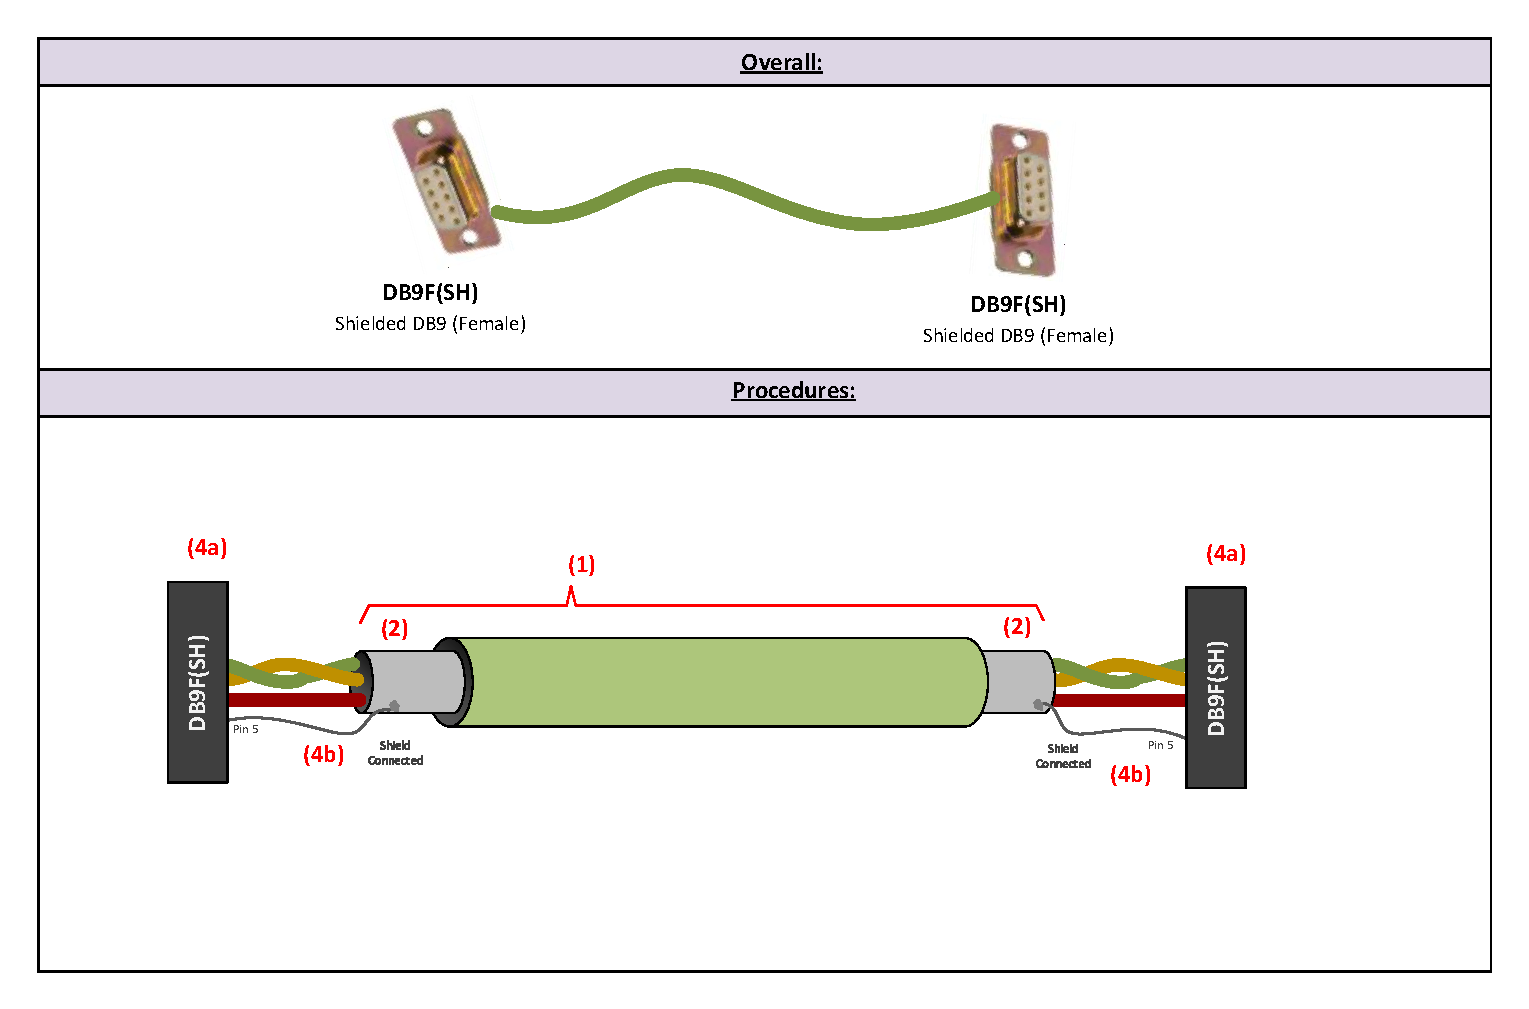
\includegraphics[angle=90,width=1\columnwidth]{figs/body03/FIGCANIIconstruction.pdf}\\
  \caption[Construction of CAN/I-I - Cable for CAN between interfaces]{Construction of CAN/I-I - Cable for CAN between interfaces}
  \label{FIG:CANIIconstruction}
\end{figure}

\subsubsection{Construction of CAN/I-PC - Cable for CAN between PC and an interface} \label{CONSTRUCTION:CANIPC}
Use figure~\ref{FIG:CANIPCconstruction} as a reference for the correct construction of this cable type. Please follow these procedures:
\begin{itemize}
  \item (1) Cut a piece of the CAN cable (described in section~\ref{CABLETYPE:CAN}) to the correct length indicated in the cable list (figure~\ref{FIG:CABLELIST}).
  \item (2) Leave a piece of cable/wire envelops striped at each cable end.
  \item (3) If an Ethernet cable is used: a) use a pair as CAN-High and CAN-Low; b) use a wire from another pair as the CAN GND; c) ignore the other wires.
  \item (4) Install the connector DB9F(SH) - Shielded DB9 (Female) at both cable sides. Use the section~\ref{DEVICE:DB9F(SH)} as a reference for pinout. Installation steps:
  \begin{itemize}
    \item a) Use the procedures described at subsection~\ref{CRIMPINGDB9} for the connector installation.
    \item b) Please note: the cable shield must be connected to the DB9 (pin 5) at both sides.
  \end{itemize}
  \item (4) Install the connector 10pinF - 10-pin for CAN (Female) at both cable sides. Use the section~\ref{DEVICE:10pinF(CAN)} as a reference for pinout. Installation steps:
  \begin{itemize}
    \item a) Use the procedures described at subsection~\ref{CRIMPING10pin} for the connector installation.
    \item b) Please note: the cable shield must be cut off near this 10-pin connector. Do not plug the shield envelopment at this side!
  \end{itemize}
\end{itemize}
\begin{figure}
  \centering
  % Requires \usepackage{graphicx}
  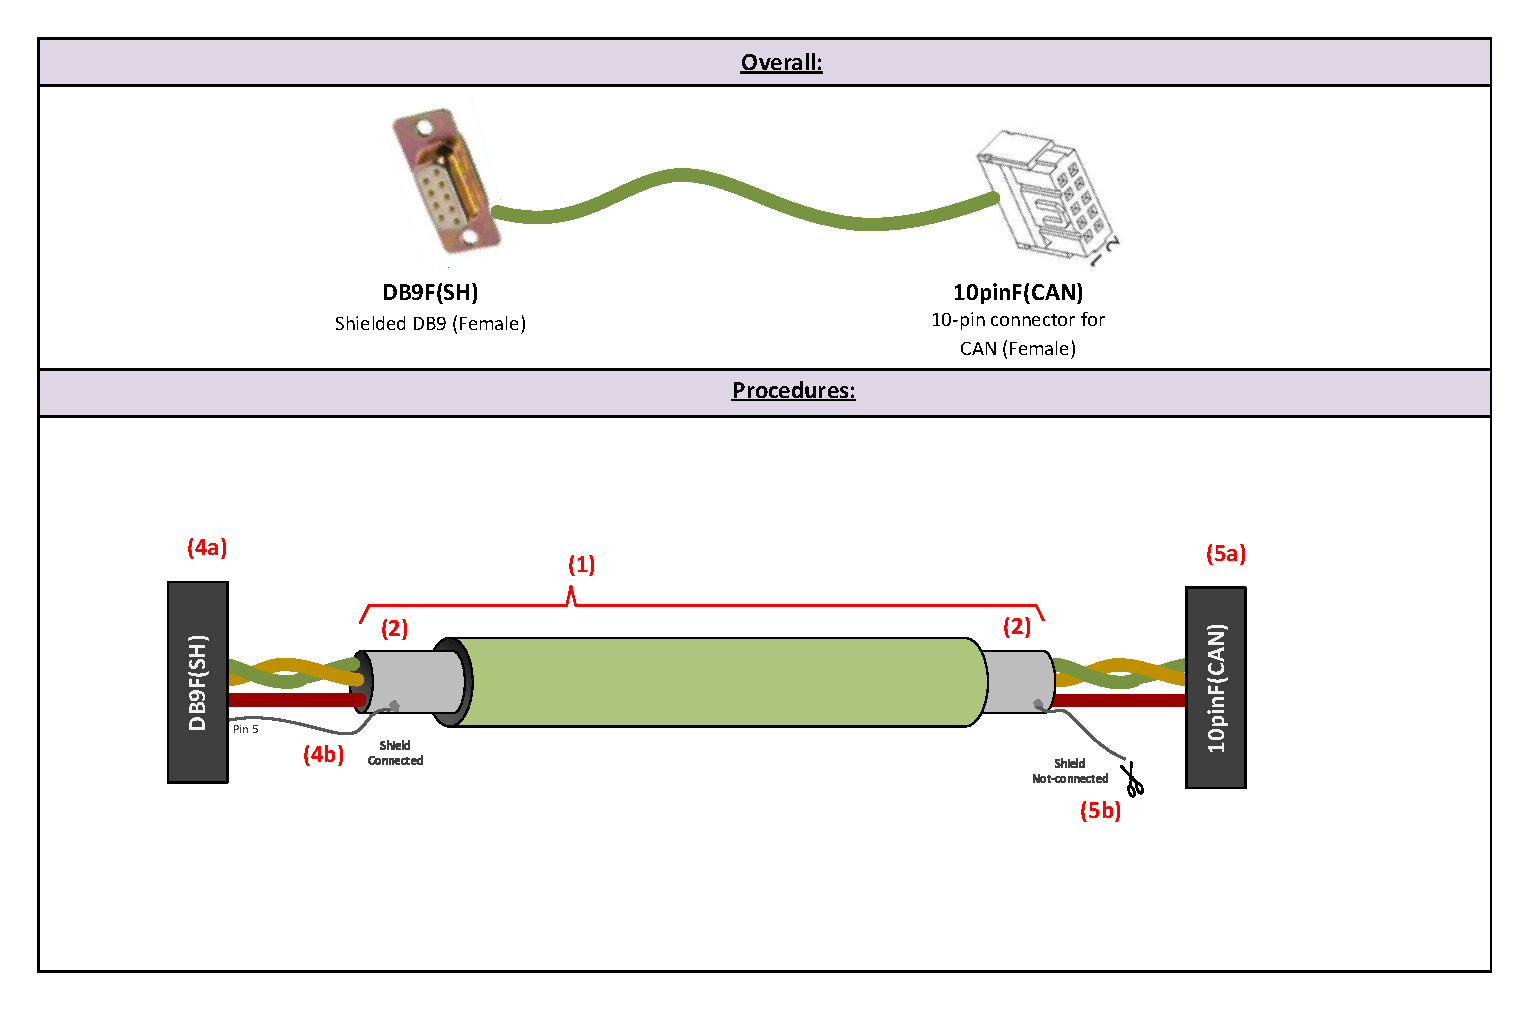
\includegraphics[angle=90,width=1\columnwidth]{figs/body03/FIGCANIPCconstruction.pdf}\\
  \caption[Construction of CAN/I-PC - Cable for CAN between PC and an interface]{Construction of CAN/I-PC - Cable for CAN between PC and an interface}
  \label{FIG:CANIPCconstruction}
\end{figure}

\subsubsection{Construction of CAN/Out - Outdoor cable for CAN between modules} \label{CONSTRUCTION:CANOut}
Use figure~\ref{FIG:CANOutconstruction} as a reference for the correct construction of this cable type. Please follow these procedures:
\begin{itemize}
  \item (1) Cut a piece of the CAN cable (described in section~\ref{CABLETYPE:CAN}) to the correct length indicated in the cable list (figure~\ref{FIG:CABLELIST}).
  \item (2) Leave a piece of cable/wire envelops striped at each cable end.
  \item (3) If an Ethernet cable is used: a) use a pair as CAN-High and CAN-Low; b) use a wire from another pair as the CAN GND; c) ignore the other wires.
  \item (4) Pass the cable inside the CAN cable gland (section~\ref{DEVICE:CG(CAN)}).
  \item (5) Install the connector DB9M(SH) - Shielded DB9 (Male) at this cable side. Use the section~\ref{DEVICE:DB9M(SH)} as a reference for pinout. Installation steps:
  \begin{itemize}
    \item a) Use the procedures described at subsection~\ref{CRIMPINGDB9} for the connector installation.
    \item b) Please note: the cable shield must be connected to this DB9 (pin 5).
  \end{itemize}
  \item (6) Install the connector SCANM(SH) - Shielded Special CAN Industrial Connector (Male) at this cable side. Use the section~\ref{DEVICE:SCANM(SH)} as a reference for pinout. Installation steps:
  \begin{itemize}
    \item a) Use the procedures described at subsection~\ref{CRIMPING4pin} for the connector installation.
    \item b) Please note: the shield must be cut off near this 4-pin connector. Do not plug the shield envelopment at this side!
  \end{itemize}
  \item (7) Once the cable is plugged into the robot rear interface, the cable gland must be installed at the specific hole on the module chassis rear. Then, the cable gland must be screwed until the cable get tight enough.
\end{itemize}
\begin{figure}
  \centering
  % Requires \usepackage{graphicx}
  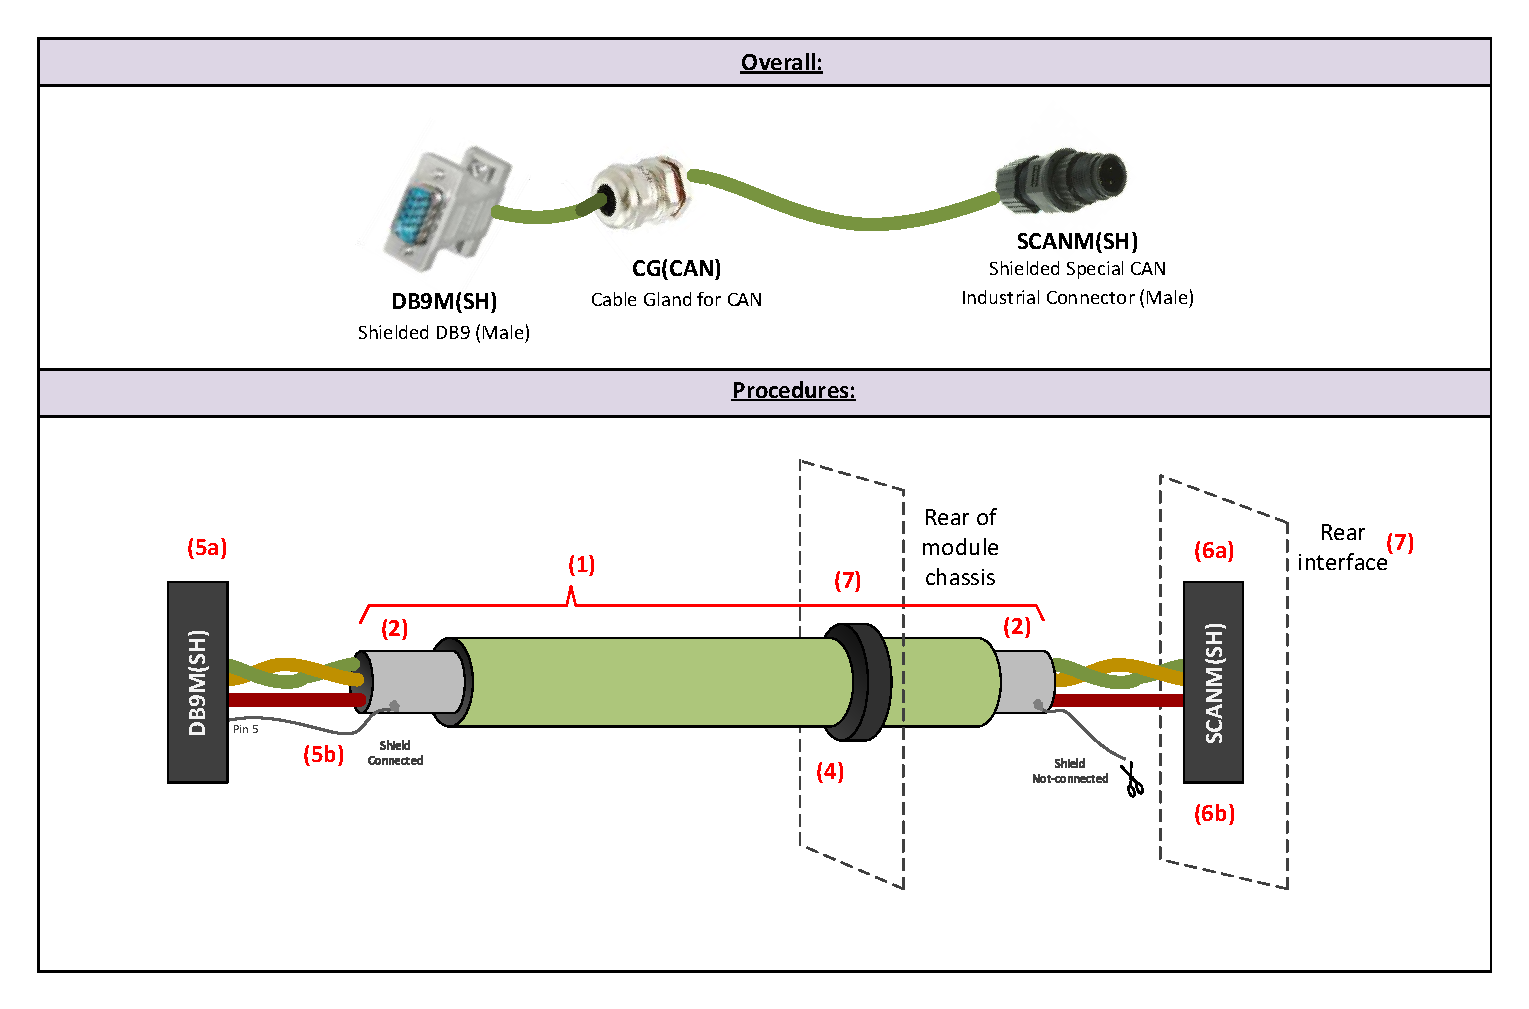
\includegraphics[angle=90,width=1\columnwidth]{figs/body03/FIGCANOutconstruction.pdf}\\
  \caption[Construction of CAN/Out - Outdoor cable for CAN between modules]{Construction of CAN/Out - Outdoor cable for CAN between modules}
  \label{FIG:CANOutconstruction}
\end{figure}
\subsubsection{Construction of LAN/I-S - Cable for Ethernet between Ethernet Switch and an interface} \label{CONSTRUCTION:LANIS}
Use figure~\ref{FIG:LANISconstruction} as a reference for the correct construction of this cable type. Please follow these procedures:
\begin{itemize}
  \item (1) Cut a piece of the CAN cable (described in section~\ref{CABLETYPE:Ethernet}) to the correct length indicated in the cable list (figure~\ref{FIG:CABLELIST}).
  \item (2) Leave a piece of cable/wire envelops striped at each cable end.
  \item (3) Install the connector RJ45M(SH) - Shielded RJ-45 (Male) at this cable side. Use the section~\ref{DEVICE:RJ45M(SH)} as a reference for pinout. Installation steps:
  \begin{itemize}
    \item a) Use the procedures described at subsection~\ref{CRIMPINGRJ45} for the connector installation.
    \item b) Please note: the cable shield must be connected to the RJ-45 shield at both cable sides!
  \end{itemize}
\end{itemize}
\begin{figure}
  \centering
  % Requires \usepackage{graphicx}
  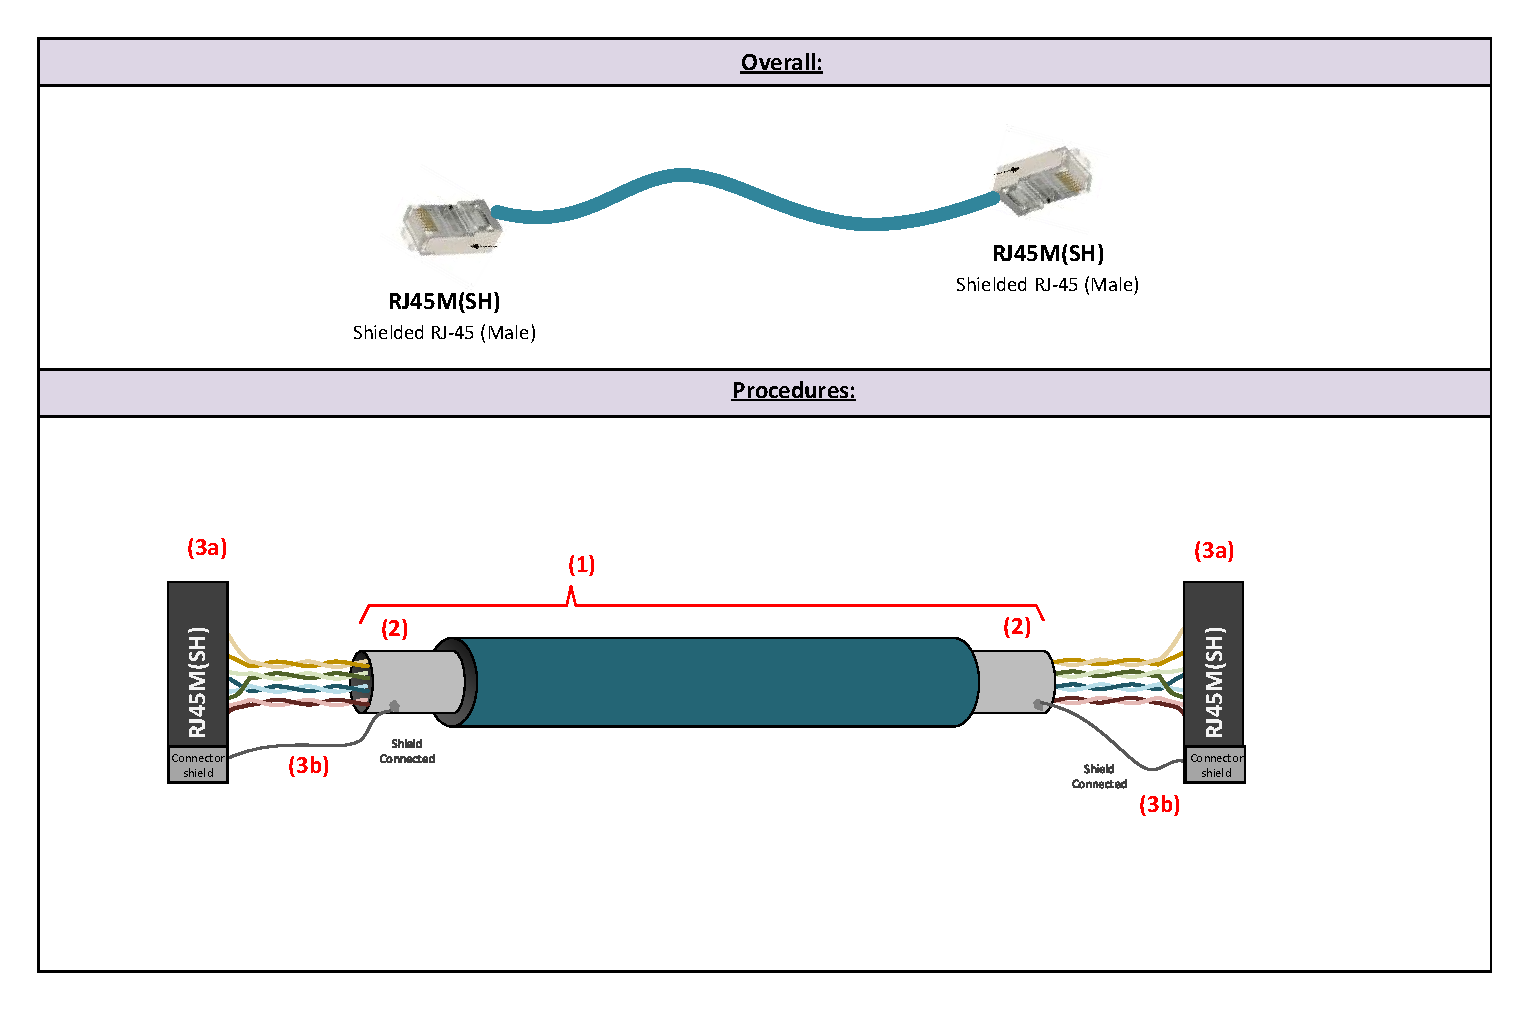
\includegraphics[angle=90,width=1\columnwidth]{figs/body03/FIGLANISconstruction.pdf}\\
  \caption[Construction of LAN/I-S - Cable for Ethernet between Ethernet Switch and an interface]{Construction of LAN/I-S - Cable for Ethernet between Ethernet Switch and an interface}
  \label{FIG:LANISconstruction}
\end{figure}

\subsubsection{Construction of LAN/Out - Outdoor cable for Ethernet between modules} \label{CONSTRUCTION:LANOut}
Use figure~\ref{FIG:LANOutconstruction} as a reference for the correct construction of this cable type. Please follow these procedures:
\begin{itemize}
  \item (1) Cut a piece of the CAN cable (described in section~\ref{CABLETYPE:Ethernet}) to the correct length indicated in the cable list (figure~\ref{FIG:CABLELIST}).
  \item (2) Leave a piece of cable/wire envelops striped at each cable end.
  \item (3) Pass the cable inside the Ethernet cable gland (section~\ref{DEVICE:CG(LAN)}).
  \item (4) Install the connector RJ45M(SH) - Shielded RJ-45 (Male) at this cable side. Use the section~\ref{DEVICE:RJ45M(SH)} as a reference for pinout. Installation steps:
  \begin{itemize}
    \item a) Use the procedures described at subsection~\ref{CRIMPINGRJ45} for the connector installation.
    \item b) Please note: the cable shield must be connected to the the shield of this RJ45.
  \end{itemize}
  \item (5) Install the connector SLANM(SH) - Shielded Special Ethernet Industrial Connector (Male) at this cable side. Use the section~\ref{DEVICE:SLANM(SH)} as a reference for pinout. Installation steps:
  \begin{itemize}
    \item a) Use the procedures described at subsection~\ref{CRIMPINGRJ45} for the connector installation.
    \item b) Please note: the cable shield must be cut off near this RJ45 connector. Do not plug the shield envelopment at this side!
  \end{itemize}
  \item (6) Once the cable is plugged into the robot rear interface, the cable gland must be installed at the specific hole on the module chassis rear. Then, the cable gland must be screwed until the cable get tight enough.
\end{itemize}
\begin{figure}
  \centering
  % Requires \usepackage{graphicx}
  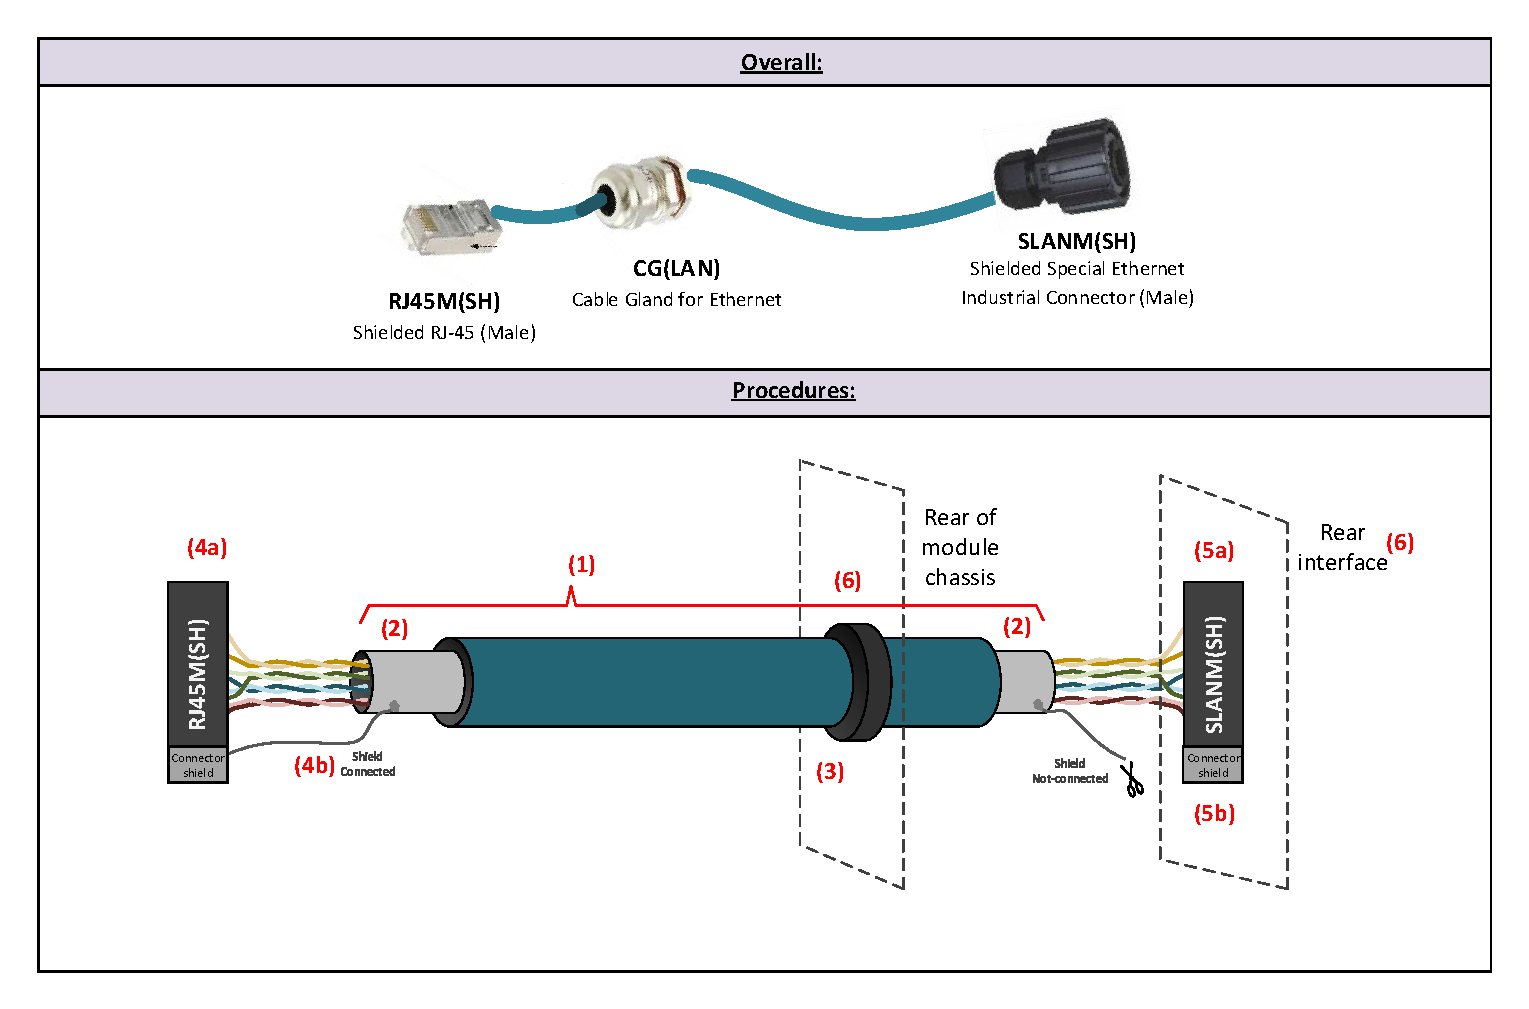
\includegraphics[angle=90,width=1\columnwidth]{figs/body03/FIGLANOutconstruction.pdf}\\
  \caption[Construction of LAN/Out - Outdoor cable for Ethernet between modules]{Construction of LAN/Out - Outdoor cable for Ethernet between modules}
  \label{FIG:LANOutconstruction}
\end{figure}
\subsubsection{Construction of LAN/S-D - Cable for Ethernet between Ethernet Switch and a device} \label{CONSTRUCTION:LANSD}
Use figure~\ref{FIG:LANSDconstruction} as a reference for the correct construction of this cable type. Please follow these procedures:
\begin{itemize}
  \item (1) Cut a piece of the CAN cable (described in section~\ref{CABLETYPE:Ethernet}) to the correct length indicated in the cable list (figure~\ref{FIG:CABLELIST}).
  \item (2) Leave a piece of cable/wire envelops striped at each cable end.
  \item (3) Install the connector RJ45M(SH) - Shielded RJ-45 (Male) at this cable side. Use the section~\ref{DEVICE:RJ45M(SH)} as a reference for pinout. Installation steps:
  \begin{itemize}
    \item a) Use the procedures described at subsection~\ref{CRIMPINGRJ45} for the connector installation.
    \item b) Please note: the cable shield must be connected to the RJ-45 shield at only one cable side!
    \item c) At the other side, please cut off the shield near the RJ-45 connector!
  \end{itemize}
\end{itemize}
\begin{figure}
  \centering
  % Requires \usepackage{graphicx}
  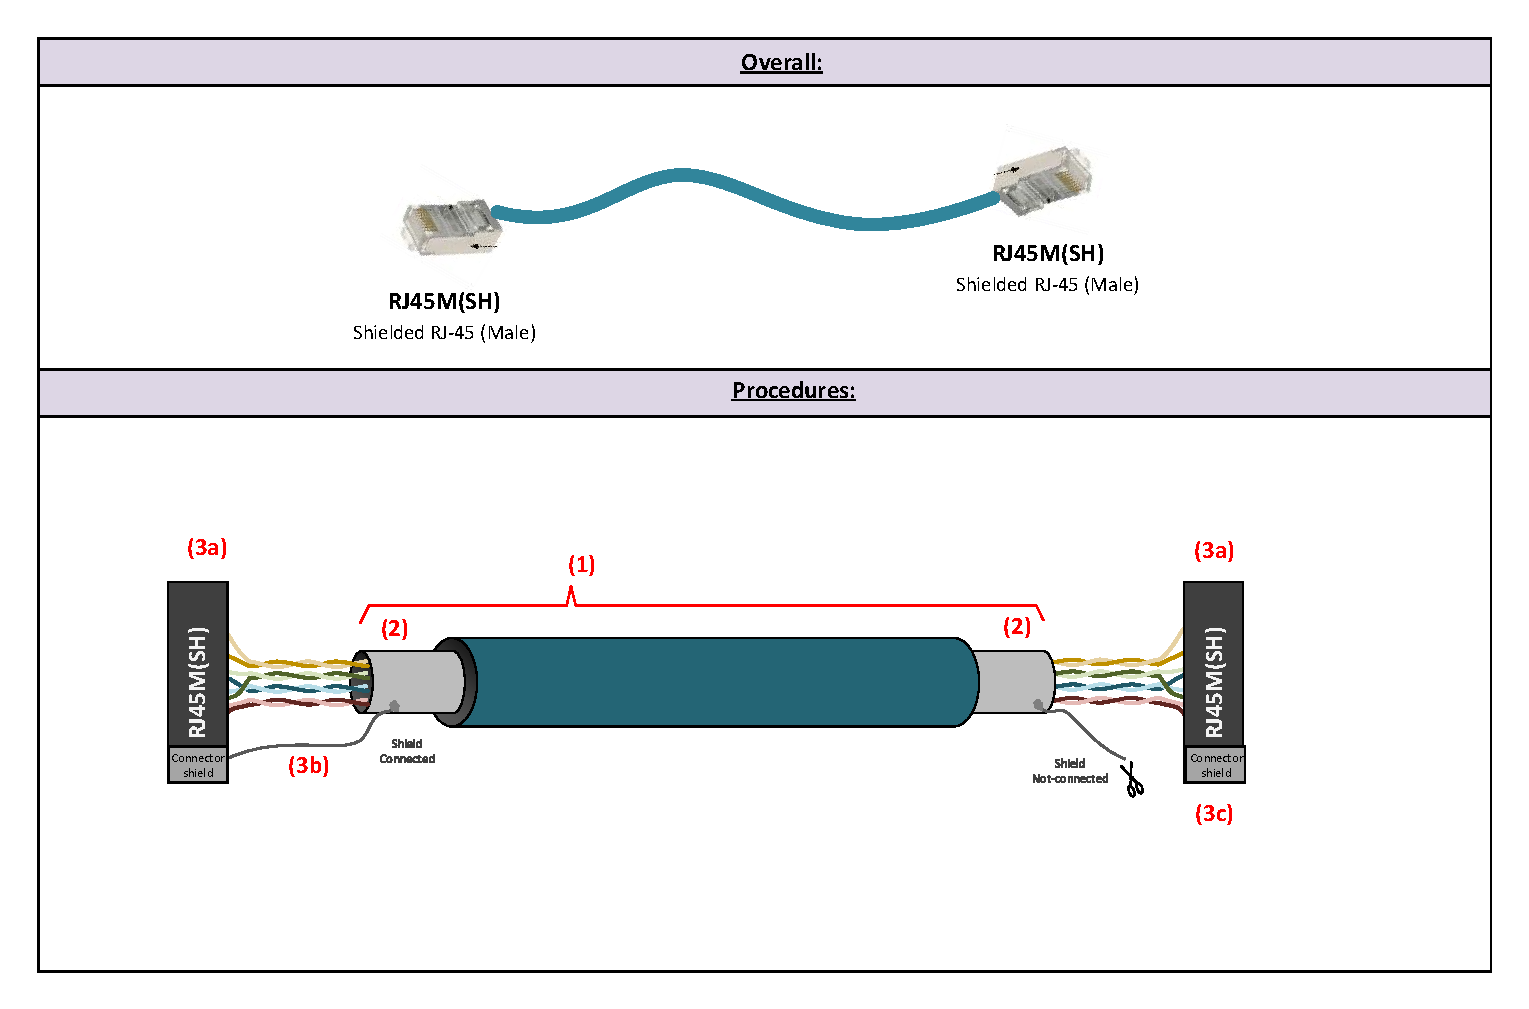
\includegraphics[angle=90,width=1\columnwidth]{figs/body03/FIGLANSDconstruction.pdf}\\
  \caption[Construction of LAN/S-D - Cable for Ethernet between Ethernet Switch and a device]{Construction of LAN/S-D - Cable for Ethernet between Ethernet Switch and a device}
  \label{FIG:LANSDconstruction}
\end{figure}

\subsubsection{Construction of USB/DAQ - Cable for USB between DAQ and PC} \label{CONSTRUCTION:USBDAQ}
The USB/DAQ cable type is provided as an accessory of DAQ. However, if needed, this cable can be purchased apart. Generally, 1 meter USB commercial cables can be easily found. Please, specify a cable with: a) USB-A connector type at one side; b) USB-B connector type at the other side. Use figure~\ref{FIG:USBDAQconstruction} as an illustration.
\begin{figure}
  \centering
  % Requires \usepackage{graphicx}
  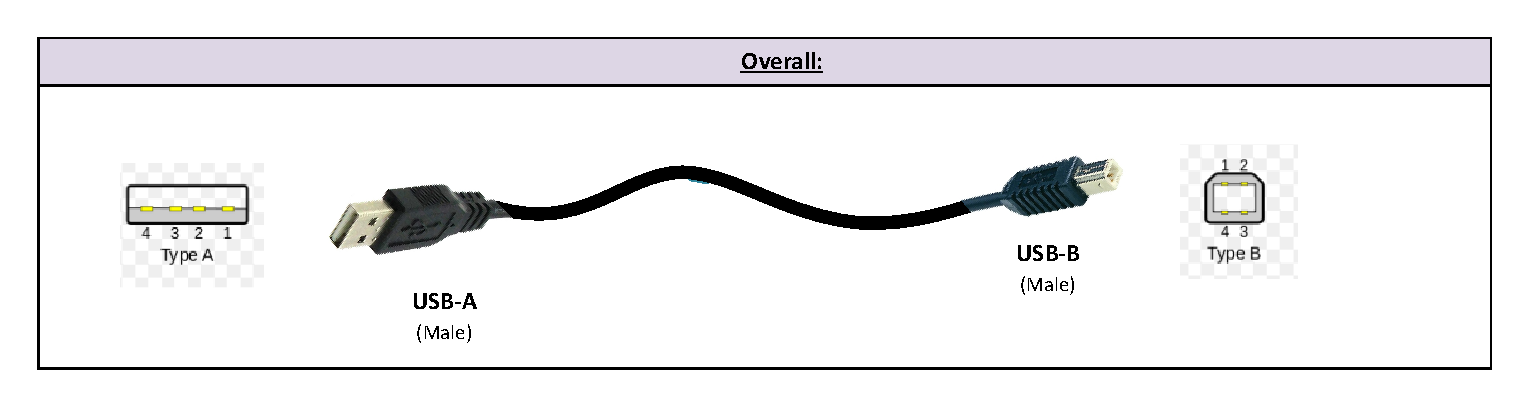
\includegraphics[angle=90,width=1\columnwidth]{figs/body03/FIGUSBDAQconstruction.pdf}\\
  \caption[USB/DAQ - Cable for USB between DAQ and PC]{USB/DAQ - Cable for USB between DAQ and PC}
  \label{FIG:USBDAQconstruction}
\end{figure}

\subsection{Connector installation procedures}
\subsubsection{Installation of 4-pin connector} \label{CRIMPING4pin}
\subsubsection{Installation of 10-pin connector} \label{CRIMPING10pin}
\subsubsection{Installation of DB9 connector family} \label{CRIMPINGDB9}
For connecting cables to DB9 type connectors (sections~\ref{DEVICE:DB9M(SH)} and~\ref{DEVICE:DB9F(SH)}), you need to perform the following steps (for both male and female types). Use figure~\ref{FIG:CRIMPDB9} as a reference.
\begin{enumerate}
  \item (1) Note that both male and female connectors are composed by a small "front panel" with small pins (male) or receptacles (females). The "rear panel" of both types is composed by special pins, in which the cable wires must be soldered.
  \item (2) Strip about 2cm of the cable envelop. For each wire to be connected, use a cutting plier (like the one described in section~\ref{DEVICE:TOOLPLIERCUTTING}) to strip the wire envelop, leaving about 2mm copper exposed.
  \item (3) Using a preheated soldering station (like the one presented in section~\ref{DEVICE:TOOLSOLDERINGSTATION}), tin the 2mm striped copper of each wire.
  \item (4) For each wire, use the correct pinout for your application (which can be checked in section~\ref{DEVICE:CONNECTORS}) and follow these steps:
  \begin{itemize}
    \item a) Place the tip inside the soldering pin.
    \item b) Using the preheated soldering station, touch the iron tip over the pin for long enough until the wire tin gets melted, and hence solded on the DB9 pin.
    \item c) Make sure that the soldered copper is entirely inside the DB9 pin.
  \item (5) Accommodate the cable inside the DB9 enclosure and close it.
  \end{itemize}
\end{enumerate}
\begin{figure}
  \centering
  % Requires \usepackage{graphicx}
  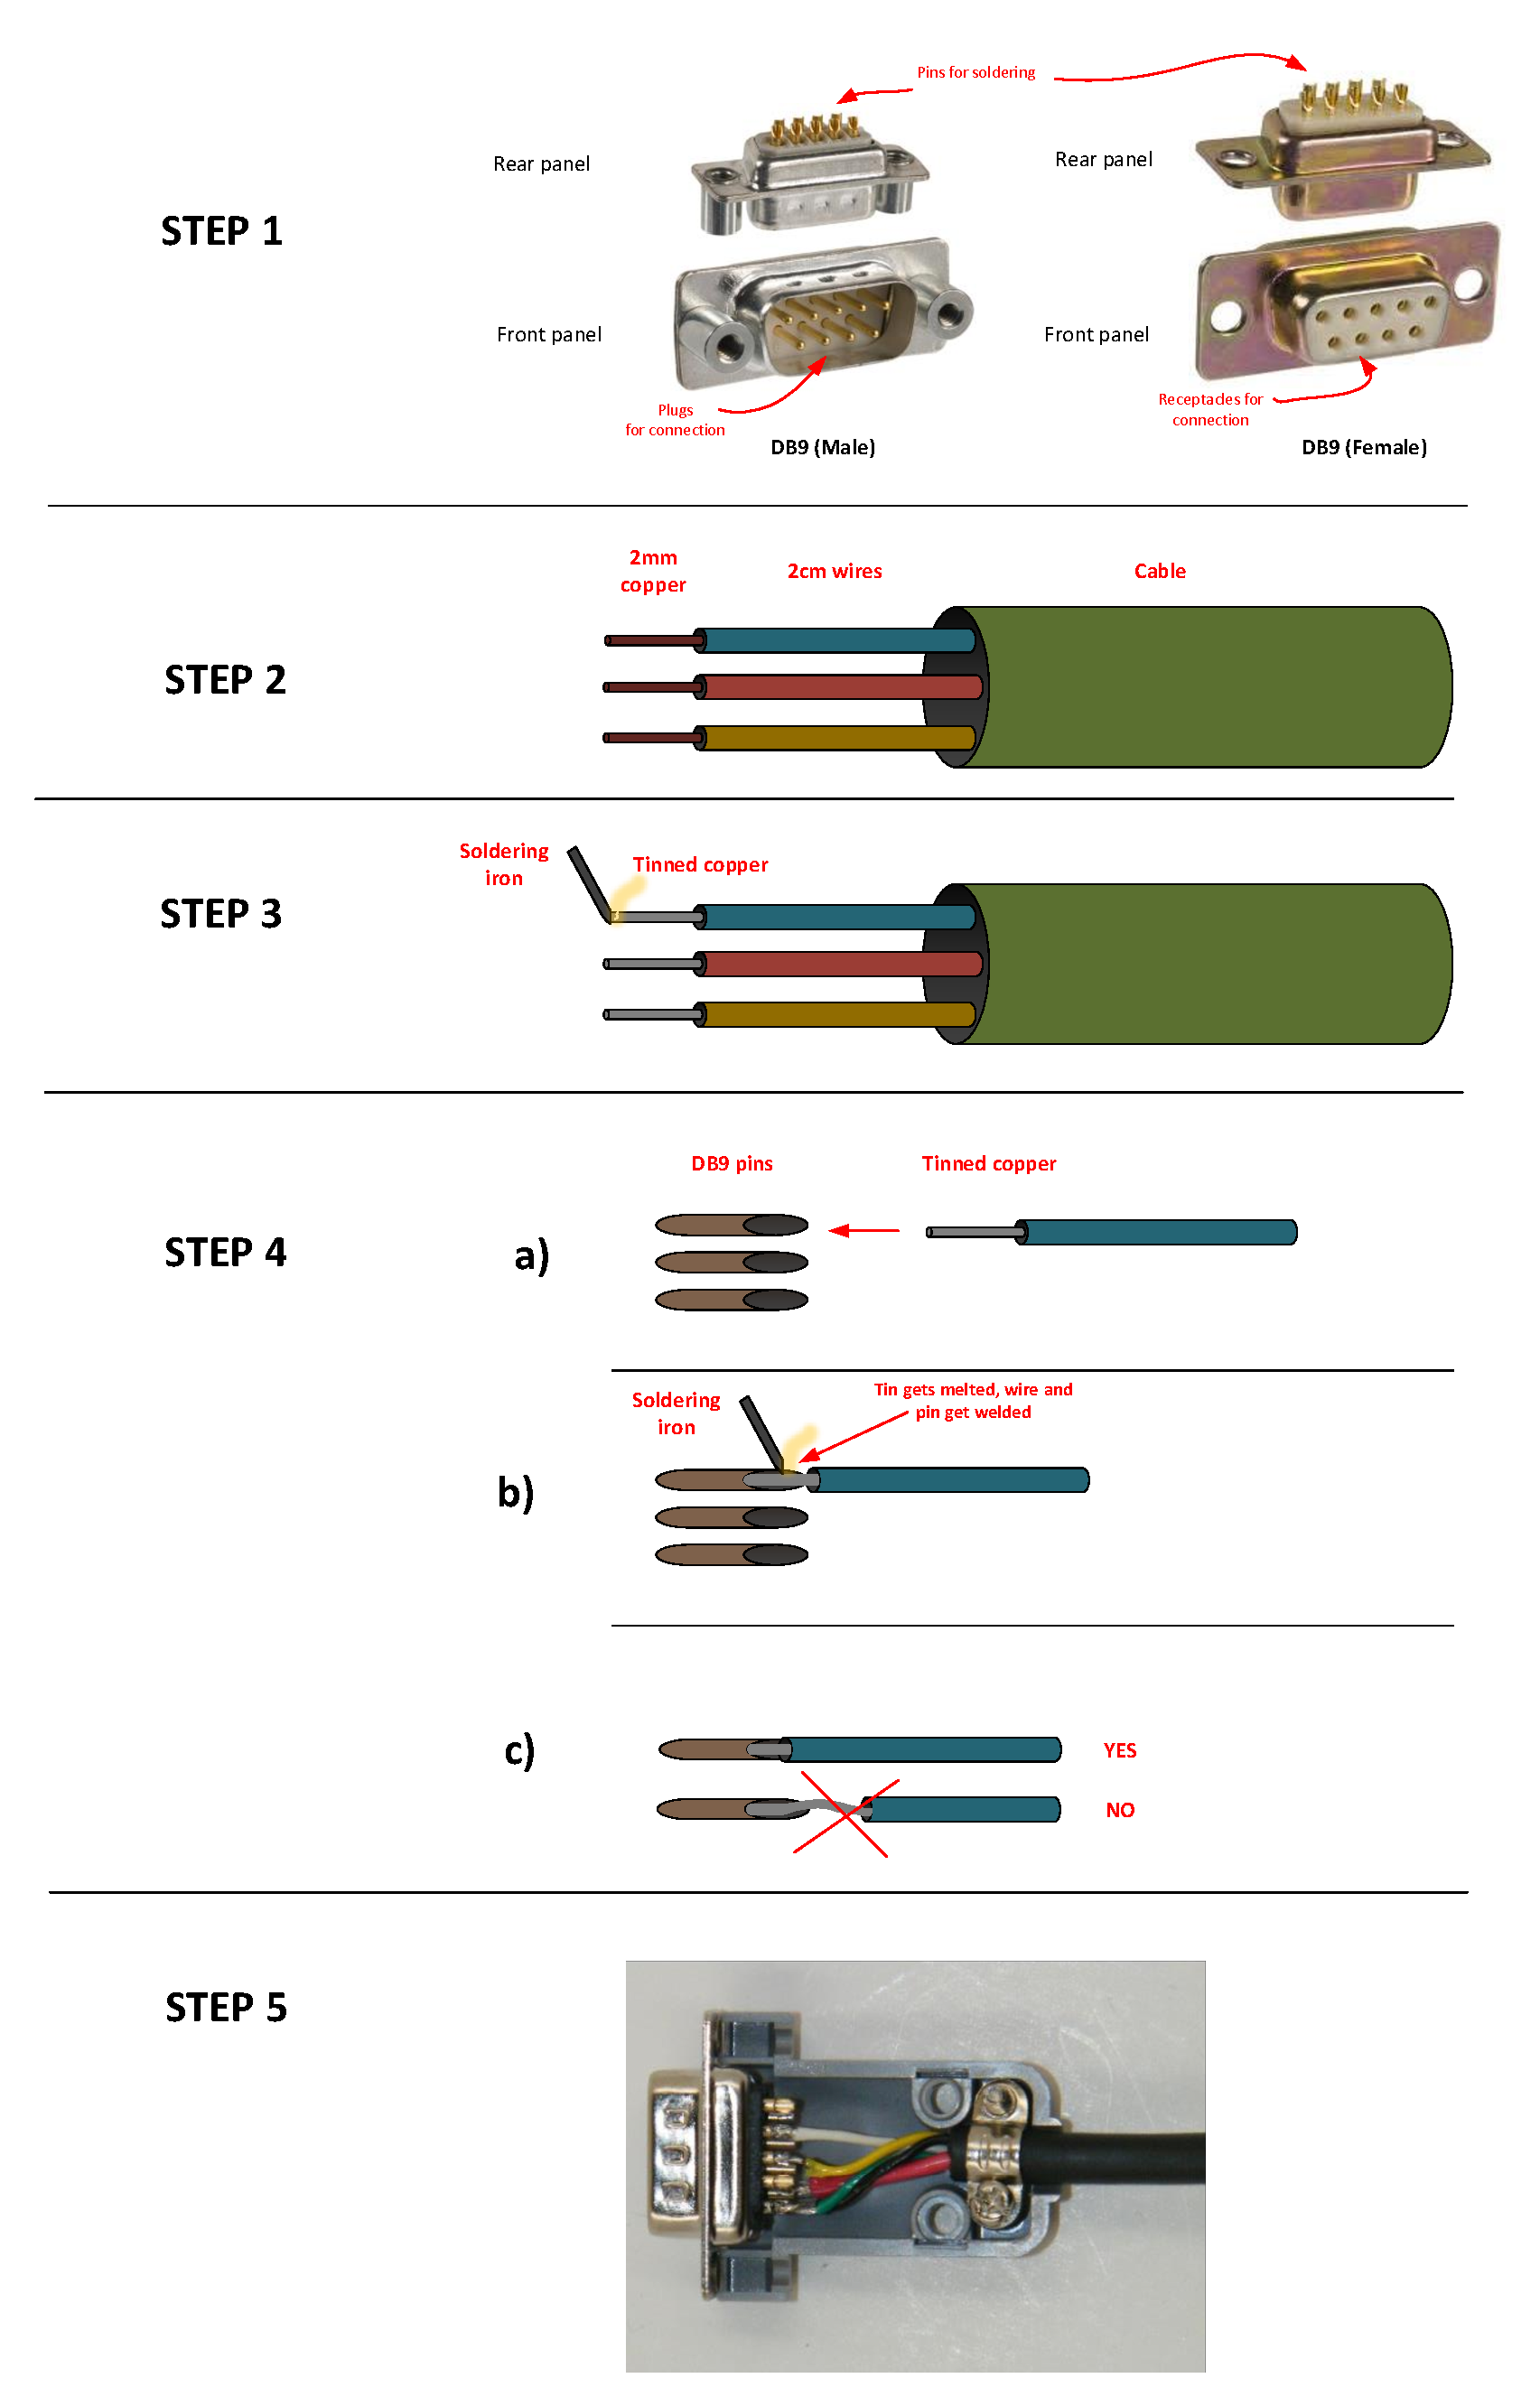
\includegraphics[angle=90,width=1\columnwidth]{figs/body03/FIGCRIMPDB9.pdf}\\
  \caption[Installation of DB9 connector family]{Installation of DB9 connector family}
  \label{FIG:CRIMPDB9}
\end{figure}
\subsubsection{Installation of RJ-45 connector family} \label{CRIMPINGRJ45}
For connecting cables to RJ-45 type connectors (sections~\ref{DEVICE:RJ45M(SH)},~\ref{DEVICE:RJ45F(SH)},~\ref{DEVICE:SLANM(SH)} and~\ref{DEVICE:SLANF(SH)}), you need to perform the following steps. Use figure~\ref{FIG:CRIMPRJ45} as an illustration and the link~\href{http://www.wikihow.com/Crimp-Rj45}{http://www.wikihow.com/Crimp-Rj45} as a reference.
  \begin{itemize}
    \item (1) Strip 2.5 to 5.1cm of the outer envelop at the end of the cable wire by making a shallow cut in the envelop with a cutting plier (like the one described in section~\ref{DEVICE:TOOLPLIERCUTTING}).
    \item (2) Fold each pair of wires backwards to expose the cable core. Cut off the core and discard it.
    \item (3) Straighten the twisted wires using 2 pair of tweezers.
    \item (4) Arrange the untwisted wires in a row, placing them into the correct position, running from right to left, in which they will go into the RJ-45 connector. Check the right pinout at sections~\ref{DEVICE:RJ45M(SH)} or~\ref{DEVICE:SLANM(SH)}.
    \item \underline{For male type}:
    \begin{itemize}
      \item a) Trim the untwisted wires to a suitable length by holding the RJ-45 connector next to the wires.
      \item b) Insert the wires into the RJ-45 connector, making sure that they stay aligned and each color goes into its appropriate channel.
      \item c) Use the RJ-45 crimping tool (section~\ref{DEVICE:TOOLCRIMPERRJ45}) to crimp the connector to the cable by pressing the jacket and cable into the connector so that the wedge at the bottom of the connector is pressed into the jacket.
    \end{itemize}
    \item \underline{For female type}:
    \begin{itemize}
      \item a) Female RJ-45 are generally for PCB applications. The connector rear is equipped with a small chip with pins or holes (see figure~\ref{FIG:DEVICESLANF(SH)} as an example), in which the ethernet wires must be soldered.
      \item b) Please use a preheated soldering station (section~\ref{DEVICE:TOOLSOLDERINGSTATION}) to solder the wires on these pins/holes. Check the right pinout at sections~\ref{DEVICE:RJ45F(SH)} or~\ref{DEVICE:SLANF(SH)}.
    \end{itemize}
  \end{itemize}

\begin{figure}
  \centering
  % Requires \usepackage{graphicx}
  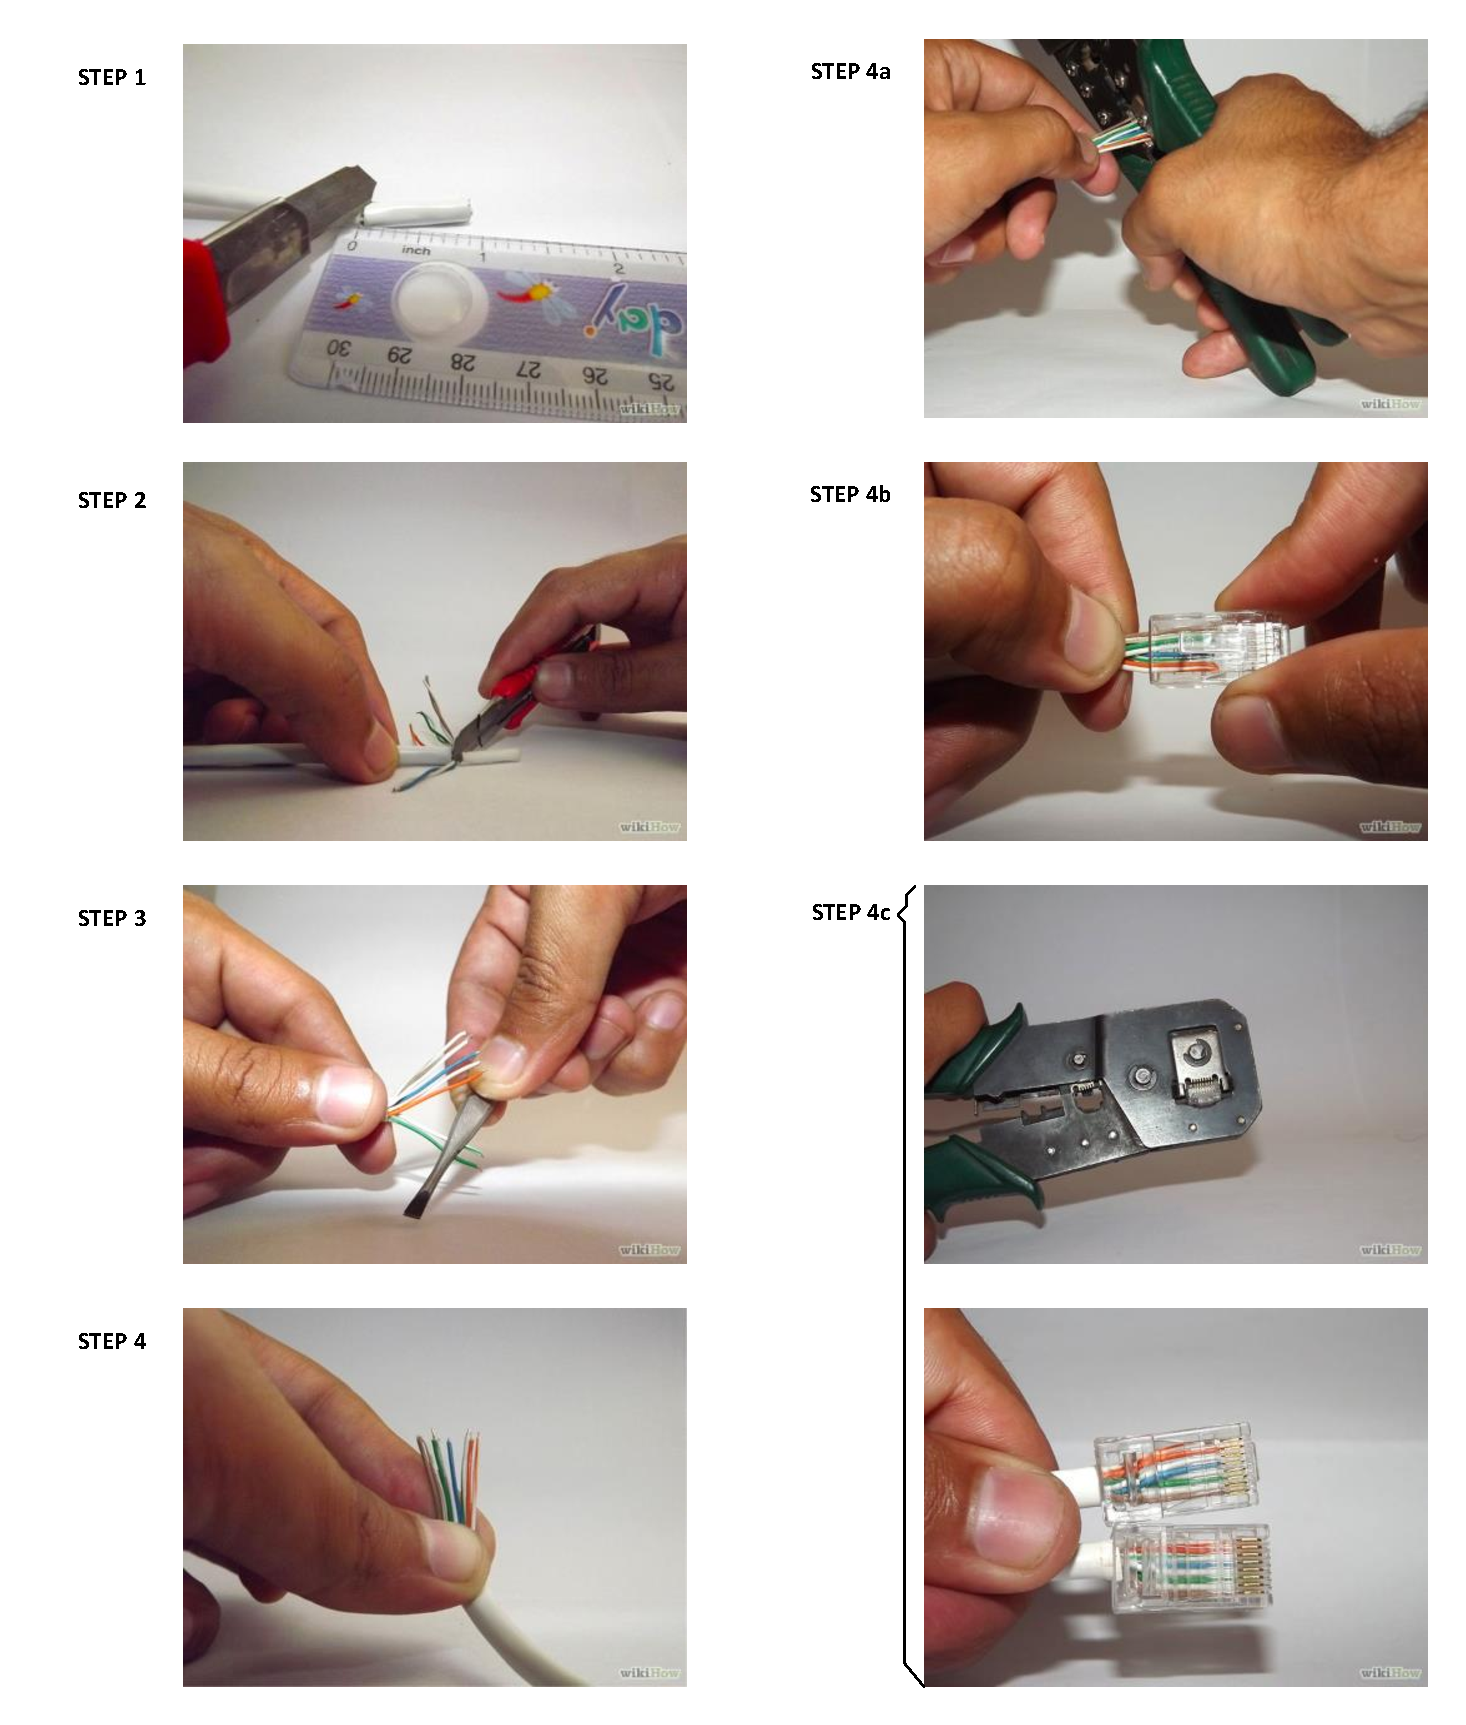
\includegraphics[angle=90,width=1\columnwidth]{figs/body03/FIGCRIMPRJ45.pdf}\\
  \caption[Installation of RJ-45 connector family]{Installation of RJ-45 connector family}
  \label{FIG:CRIMPRJ45}
\end{figure}
\subsubsection{Crimping Molex Micro-Fit 3.0\texttrademark Family} \label{CRIMPINGmicro}
For connecting wires to a Molex Micro-Fit 3.0\texttrademark connector from 43025-xxxx family (sections~\ref{DEVICE:microCAN} and~\ref{DEVICE:microHall}), you first need to crimp the edge of these wires in the Molex crimp terminal from 43030-xxxx family (section~\ref{DEVICE:microCrimp}). For this, you should perform the following steps:
\begin{enumerate}
  \item Use the tool "Molex Hand Crimper Tool Part Number: 63819-0000" (see section~\ref{DEVICE:TOOLCRIMPERmicro}).
  \item For each wire to be connected, use a cutting plier (like the one described in section~\ref{DEVICE:TOOLPLIERCUTTING}), strip the wire envelop, leaving 2mm copper exposed.
  \item Place the wire and the crimp terminal according to figure~\ref{FIG:CRIMPmicro1}.
  \item Use the Molex Hand Crimper (item 1) to crimp the wire.
  \item If the crimping tool is not available, perform these steps:
  \begin{itemize}
    \item Using a preheated soldering station (like the one presented in section~\ref{DEVICE:TOOLSOLDERINGSTATION}), tin the 2mm striped copper wire.
    \item Place the wire/crimp terminal like described in item 3.
    \item Use a long needle-nose plier (like the one presented in section~\ref{DEVICE:TOOLPLIERNEEDLENOSE}) to press the crimp flaps, following the steps described in figure~\ref{FIG:CRIMP2}.
    \item Using the preheated soldering station, touch the iron tip over the crimp terminal for long enough until the internal welding tin (on the wire tip surface) gets melted.
  \end{itemize}
  \item Repeat the previous steps for each wire.
  \item Envelop the whole wire set using 2cm of a heat shrink tube (like the ones described in section~\ref{DEVICE:TOOLTHERMALINSULATION}). Select the correct tube diameter according to your need. Use figure~\ref{FIG:CRIMP3} as a reference.
  \item Use the heat of a thermal blower (like the one described in section~\ref{DEVICE:TOOLTHERMALBLOWER}) to shrink the thermal tube around the cable/wires.
  \item Using the correct pinout for the concerning connector (which can be checked in section~\ref{DEVICE:CONNECTORS}), insert each crimped terminal into the respective connector hole. A "click" sound must be heard, and this indicates that the crimp terminal is in the correct plug position and cannot be removed. Use figure~\ref{FIG:CRIMP4} as a reference.
\end{enumerate}
\begin{figure}
  \centering
  % Requires \usepackage{graphicx}
  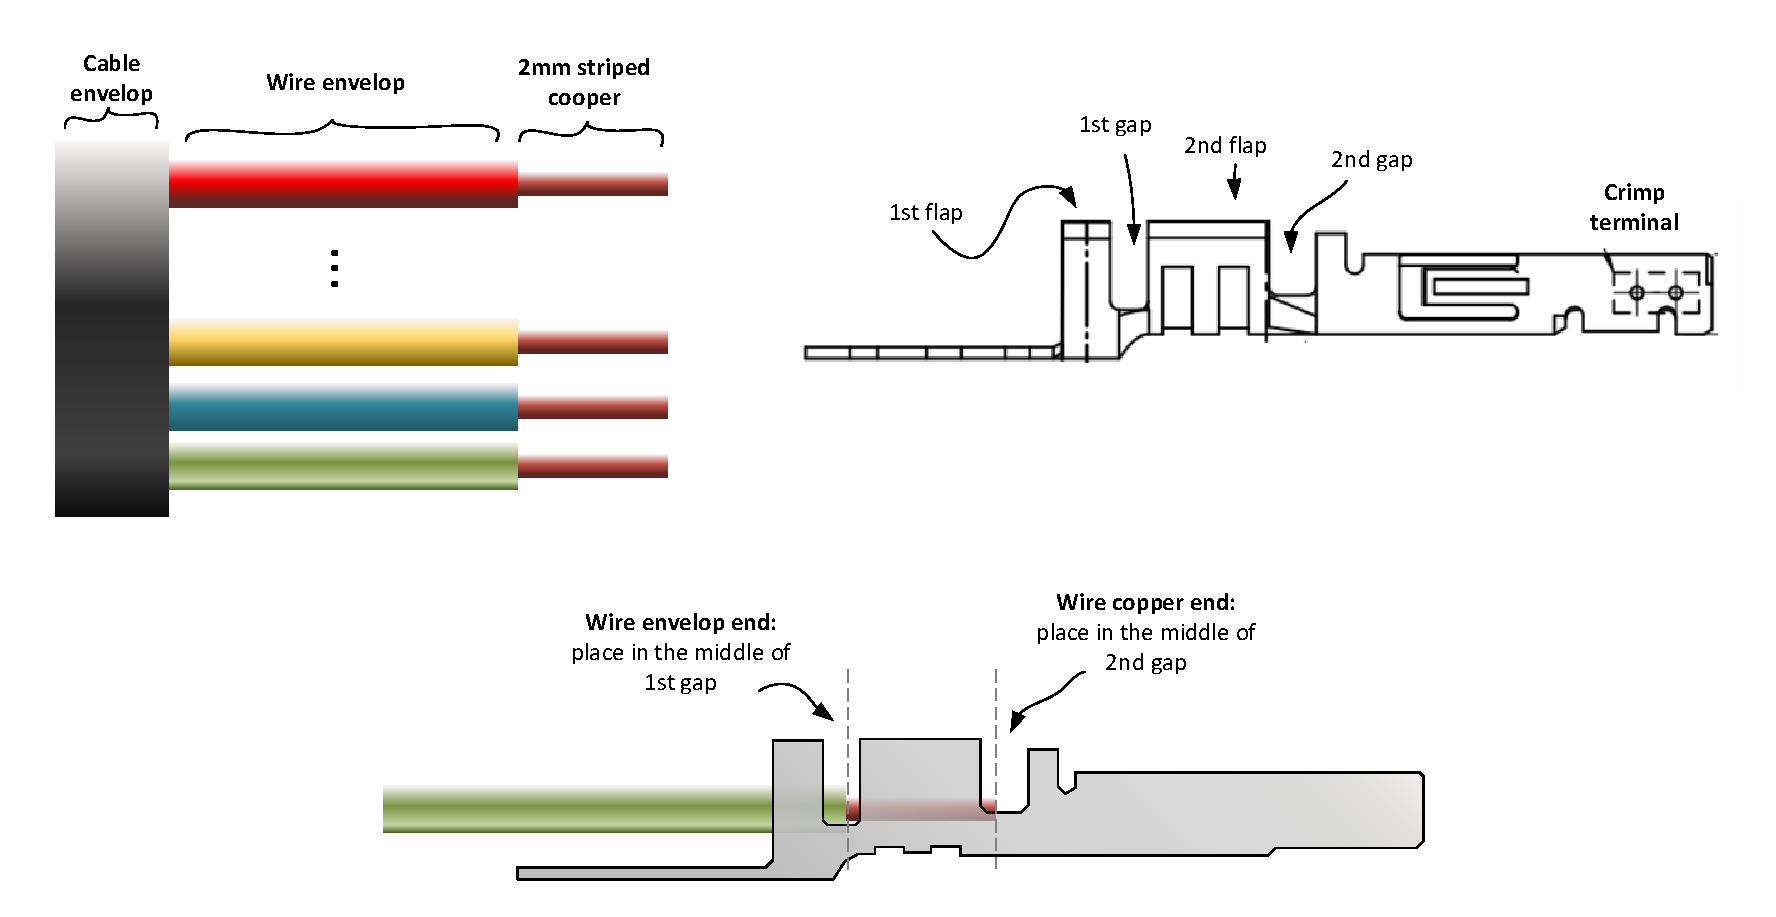
\includegraphics[angle=90,width=1\columnwidth]{figs/body03/FIGCRIMPmicro1.pdf}\\
  \caption[Crimping Molex Micro-Fit 3.0\texttrademark: placing the crimp terminal]{Crimping Molex Micro-Fit 3.0\texttrademark: placing the crimp terminal}
  \label{FIG:CRIMPmicro1}
\end{figure}
\begin{figure}
  \centering
  % Requires \usepackage{graphicx}
  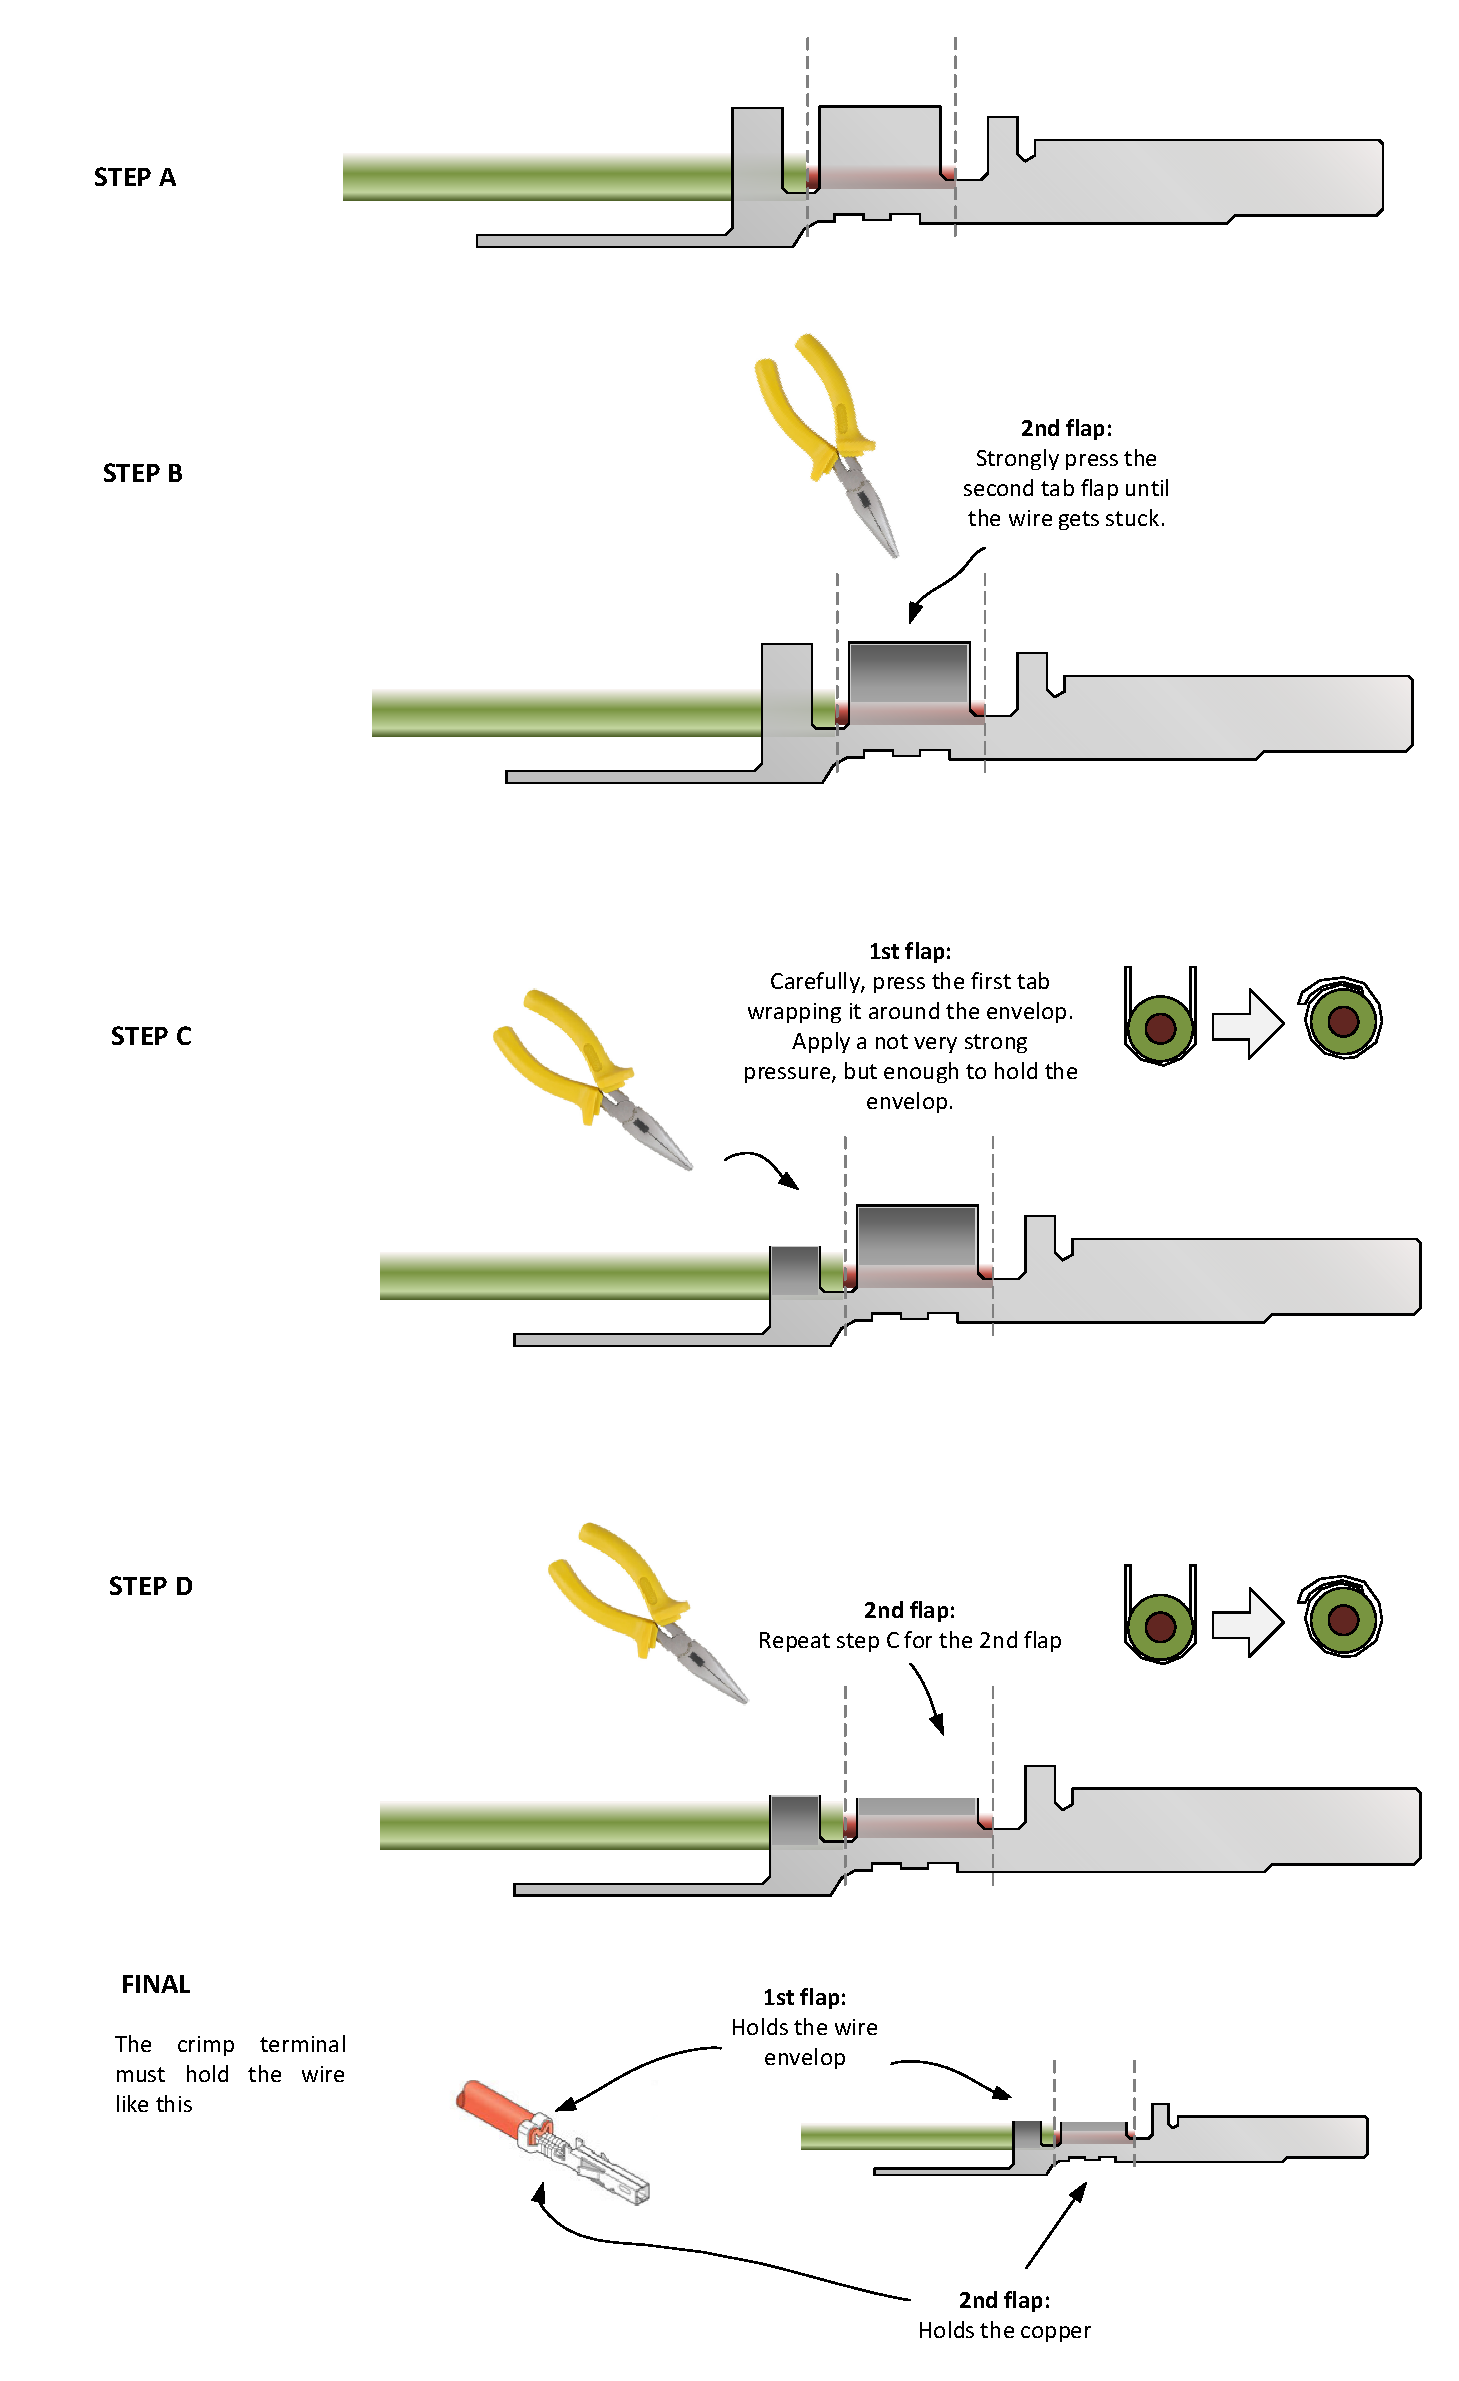
\includegraphics[angle=90,width=1\columnwidth]{figs/body03/FIGCRIMP2.pdf}\\
  \caption[Crimping Molex Micro-Fit 3.0\texttrademark: procedures for manual crimping]{Crimping Molex Micro-Fit 3.0\texttrademark: procedures for manual crimping}
  \label{FIG:CRIMP2}
\end{figure}
\begin{figure}
  \centering
  % Requires \usepackage{graphicx}
  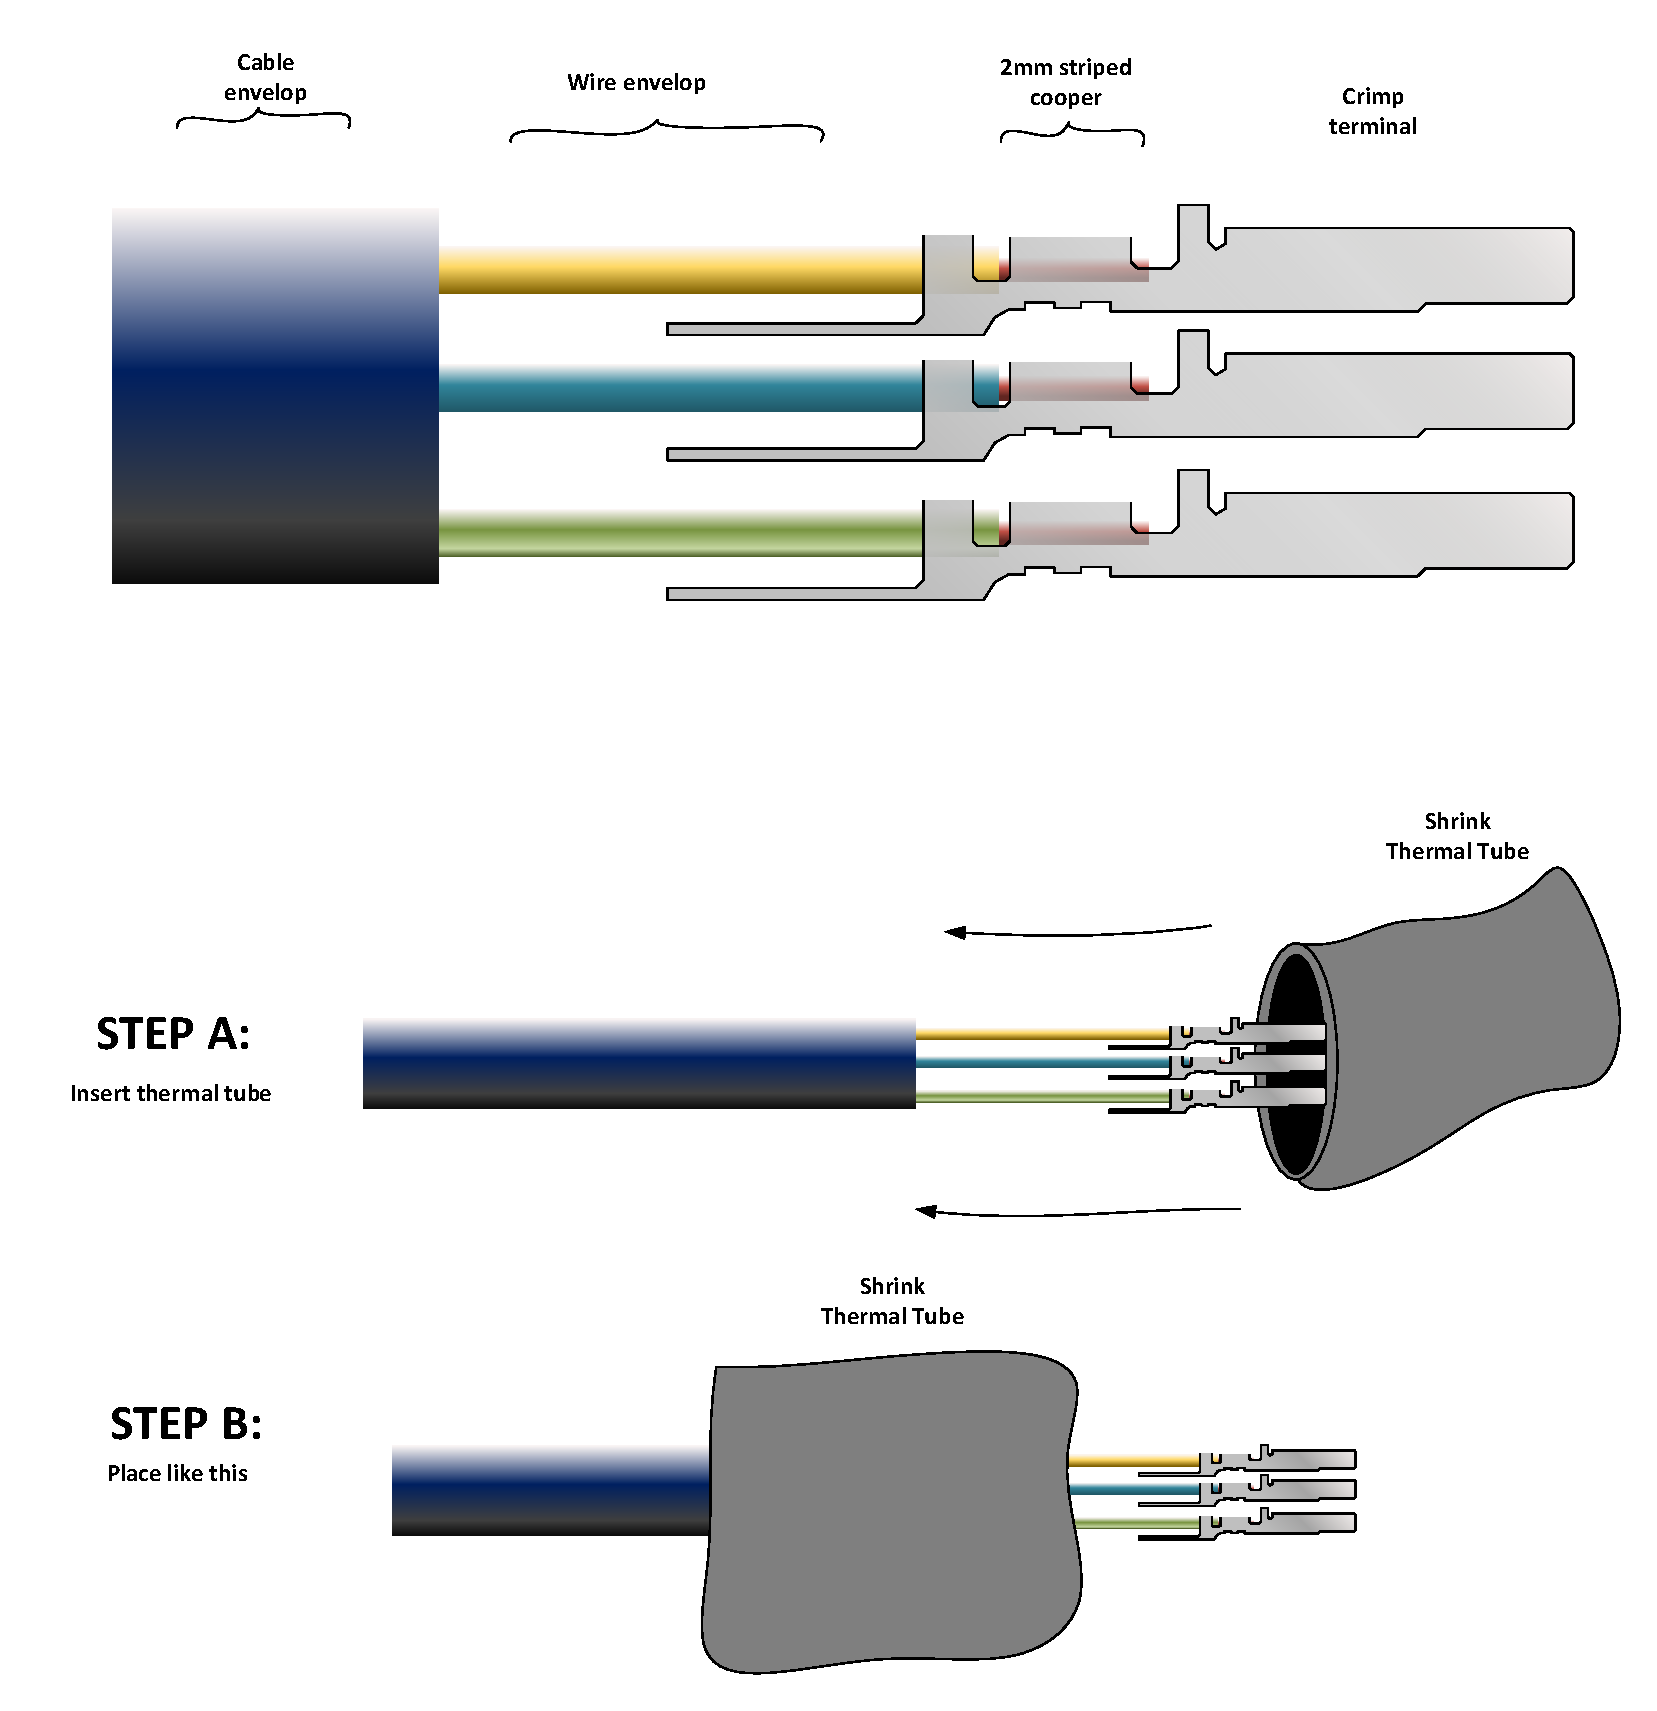
\includegraphics[angle=90,width=1\columnwidth]{figs/body03/FIGCRIMP3.pdf}\\
  \caption[Crimping Molex Micro-Fit 3.0\texttrademark: applying the heat shrink tube]{Crimping Molex Micro-Fit 3.0\texttrademark: applying the heat shrink tube}
  \label{FIG:CRIMP3}
\end{figure}
\begin{figure}
  \centering
  % Requires \usepackage{graphicx}
  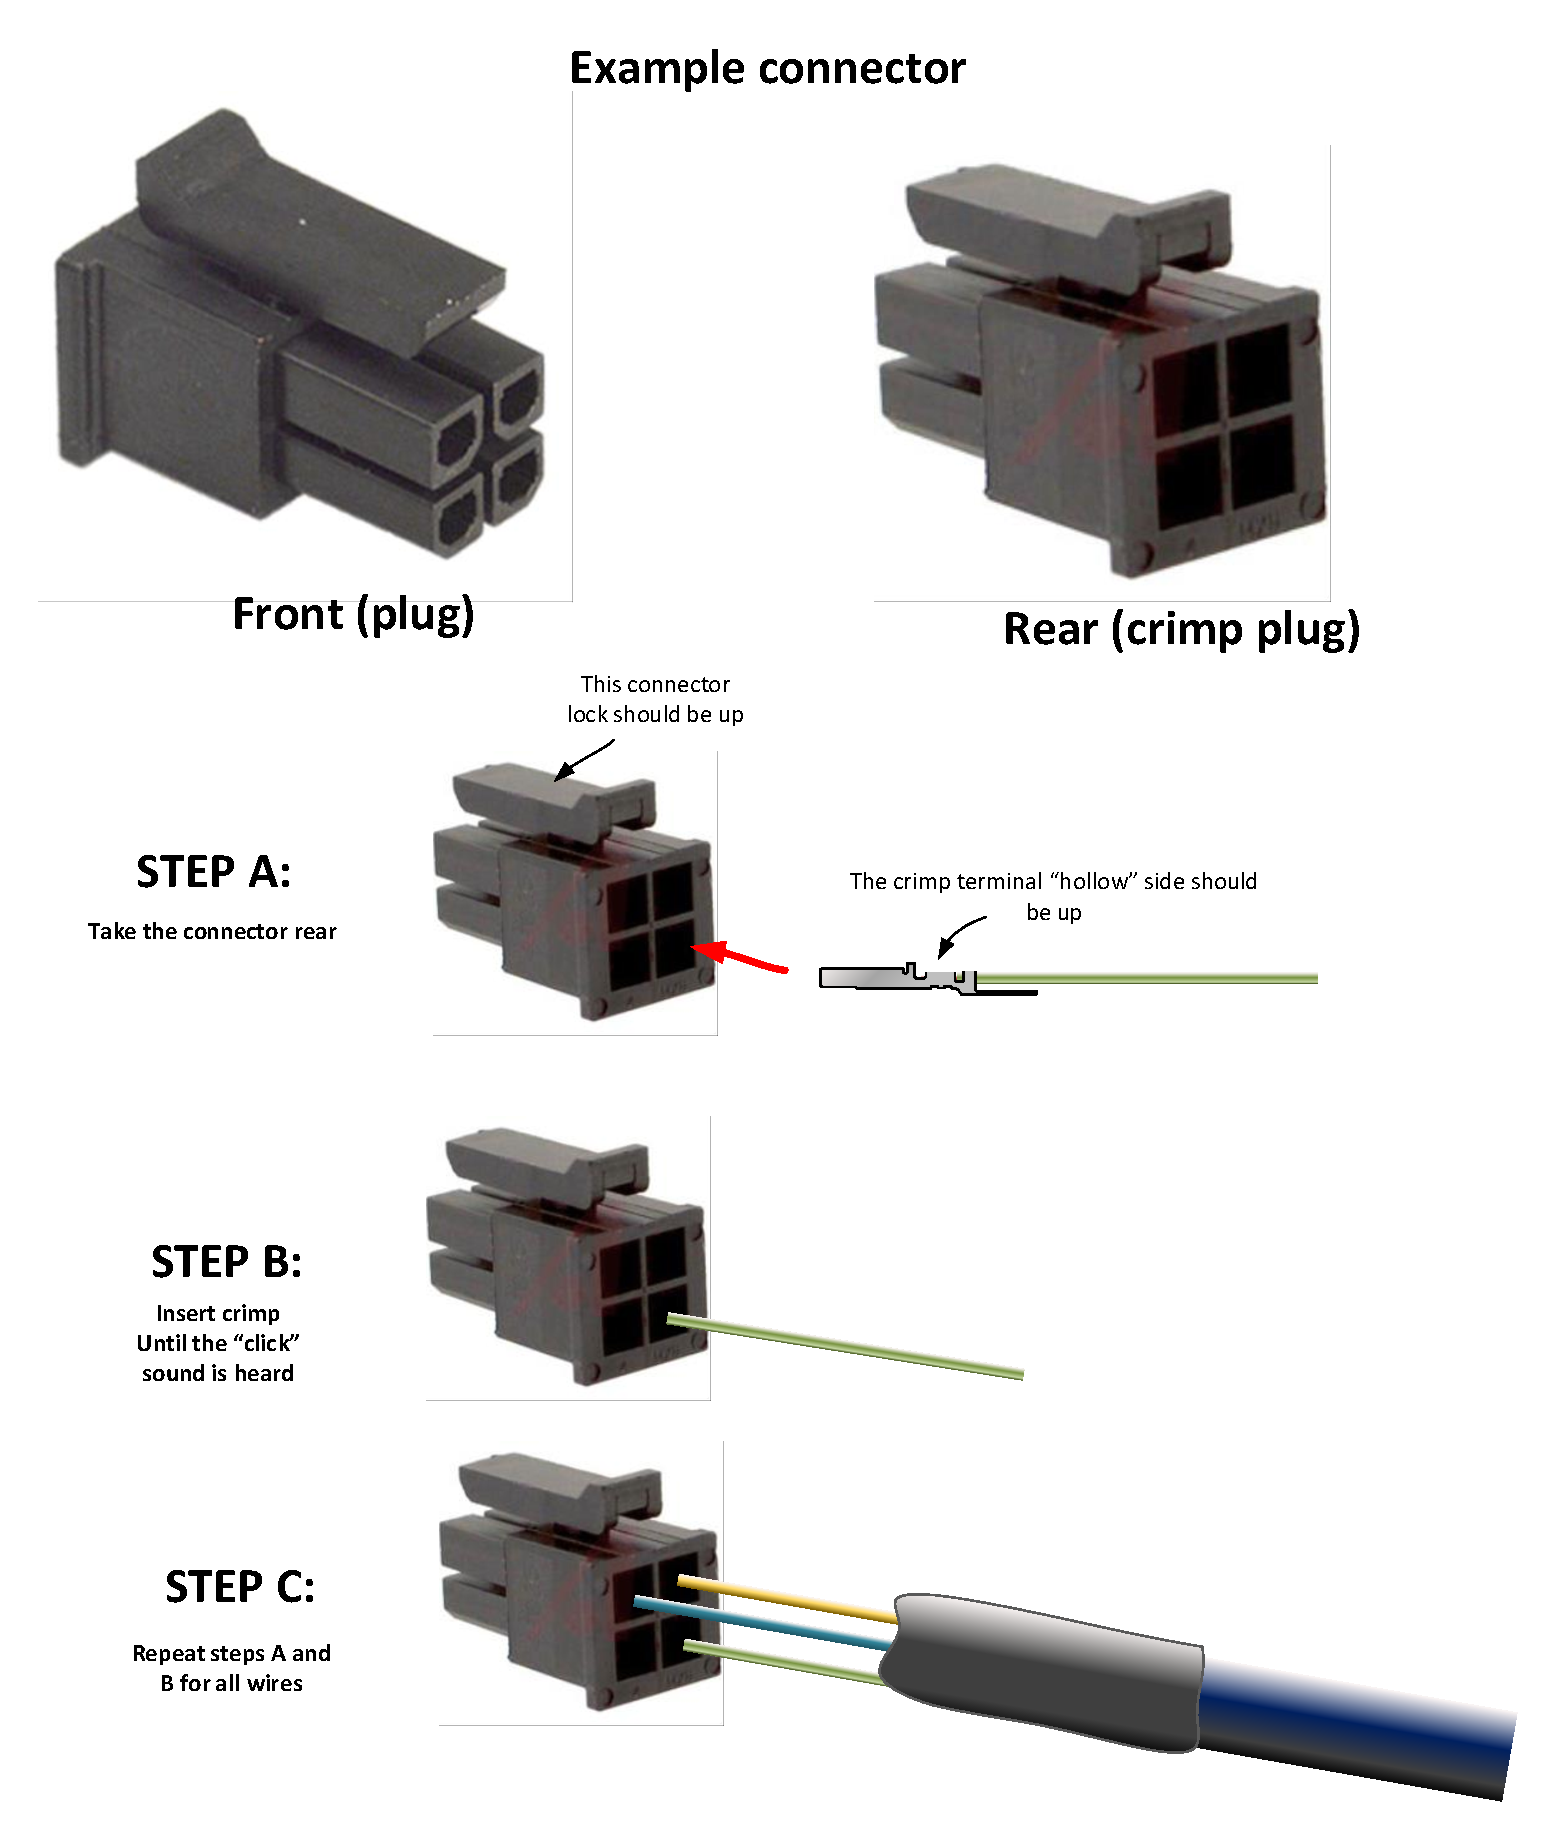
\includegraphics[angle=90,width=1\columnwidth]{figs/body03/FIGCRIMP4.pdf}\\
  \caption[Crimping Molex Micro-Fit 3.0\texttrademark: inserting the crimp terminals into the connector holes]{Crimping Molex Micro-Fit 3.0\texttrademark: inserting the crimp terminals into the connector holes}
  \label{FIG:CRIMP4}
\end{figure}
\subsubsection{Crimping Molex Mini-Fit\textregistered Family} \label{CRIMPINGmini}
For connecting wires to a Molex Mini-Fit\textregistered connector from 39-01-xxxx family (sections~\ref{DEVICE:miniMotor} and~\ref{DEVICE:miniPower}), you first need to crimp the edge of these wires in the Molex crimp terminal from 44476-xxxx family (section~\ref{DEVICE:miniCrimp}). For this, you should perform the following steps:
\begin{enumerate}
  \item Use the tool "Molex Hand Crimper Tool Part Number: 63819-0900" (see section~\ref{DEVICE:TOOLCRIMPERmini}).
  \item For each wire to be connected, use a cutting plier (like the one described in section~\ref{DEVICE:TOOLPLIERCUTTING}), strip the wire envelop, leaving 3mm copper exposed.
  \item Place the wire and the crimp terminal according to figure~\ref{FIG:CRIMPmini5}.
  \item Use the Molex Hand Crimper (item 1) to crimp the wire.
  \item If the crimping tool is not available, perform these steps:
  \begin{itemize}
    \item Using a preheated soldering station (like the one presented in section~\ref{DEVICE:TOOLSOLDERINGSTATION}), tin the 3mm striped copper wire.
    \item Place the wire/crimp terminal like described in item 3.
    \item Use a long needle-nose plier (like the one presented in section~\ref{DEVICE:TOOLPLIERNEEDLENOSE}) to press the crimp flaps, following the steps described in figure~\ref{FIG:CRIMP6}.
    \item Using the preheated soldering station, touch the iron tip over the crimp terminal for long enough until the internal welding tin (on the wire tip surface) gets melted.
  \end{itemize}
  \item Repeat the previous steps for each wire.
  \item Envelop the whole wire set using 2cm of a heat shrink tube (like the ones described in section~\ref{DEVICE:TOOLTHERMALINSULATION}). Select the correct tube diameter according to your need. Use figure~\ref{FIG:CRIMP7} as a reference.
  \item Use the heat of a thermal blower (like the one described in section~\ref{DEVICE:TOOLTHERMALBLOWER}) to shrink the thermal tube around the cable/wires.
  \item Using the correct pinout for the concerning connector (which can be checked in section~\ref{DEVICE:CONNECTORS}), insert each crimped terminal into the respective connector hole. A "click" sound must be heard, and this indicates that the crimp terminal is in the correct plug position and cannot be removed. Use figure~\ref{FIG:CRIMP8} as a reference.
\end{enumerate}
\begin{figure}
  \centering
  % Requires \usepackage{graphicx}
  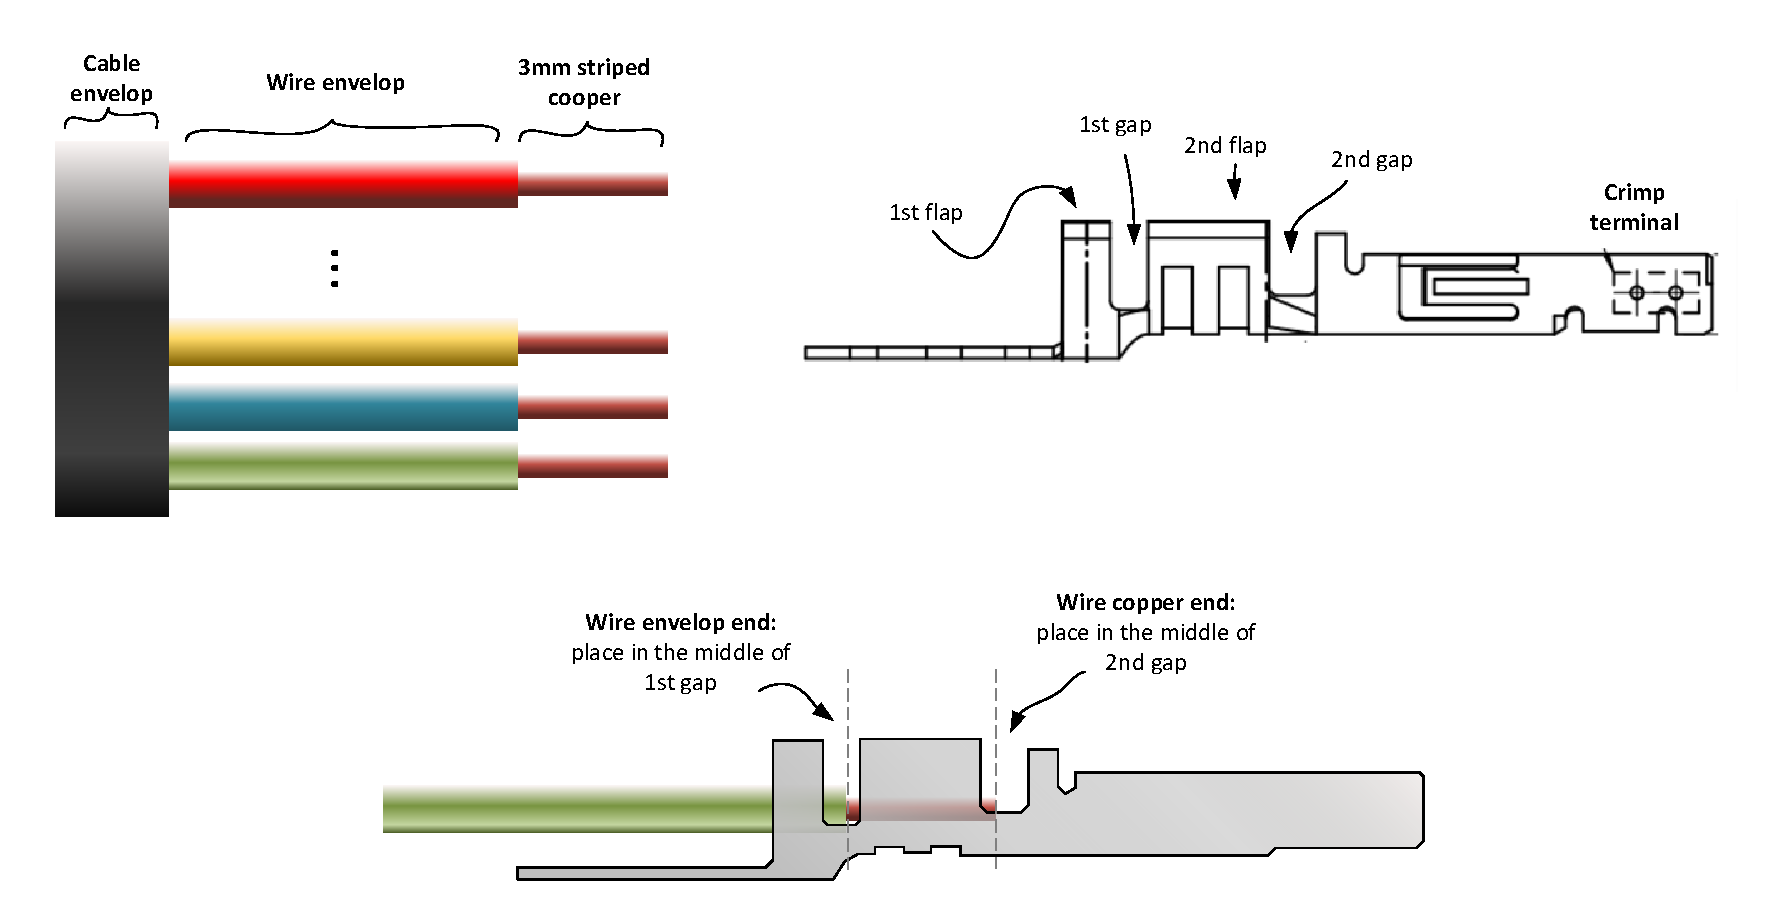
\includegraphics[angle=90,width=1\columnwidth]{figs/body03/FIGCRIMPmini5.pdf}\\
  \caption[Crimping Molex Mini-Fit \textregistered: placing the crimp terminal]{Crimping Molex Mini-Fit \textregistered: placing the crimp terminal}
  \label{FIG:CRIMPmicro5}
\end{figure}
\begin{figure}
  \centering
  % Requires \usepackage{graphicx}
  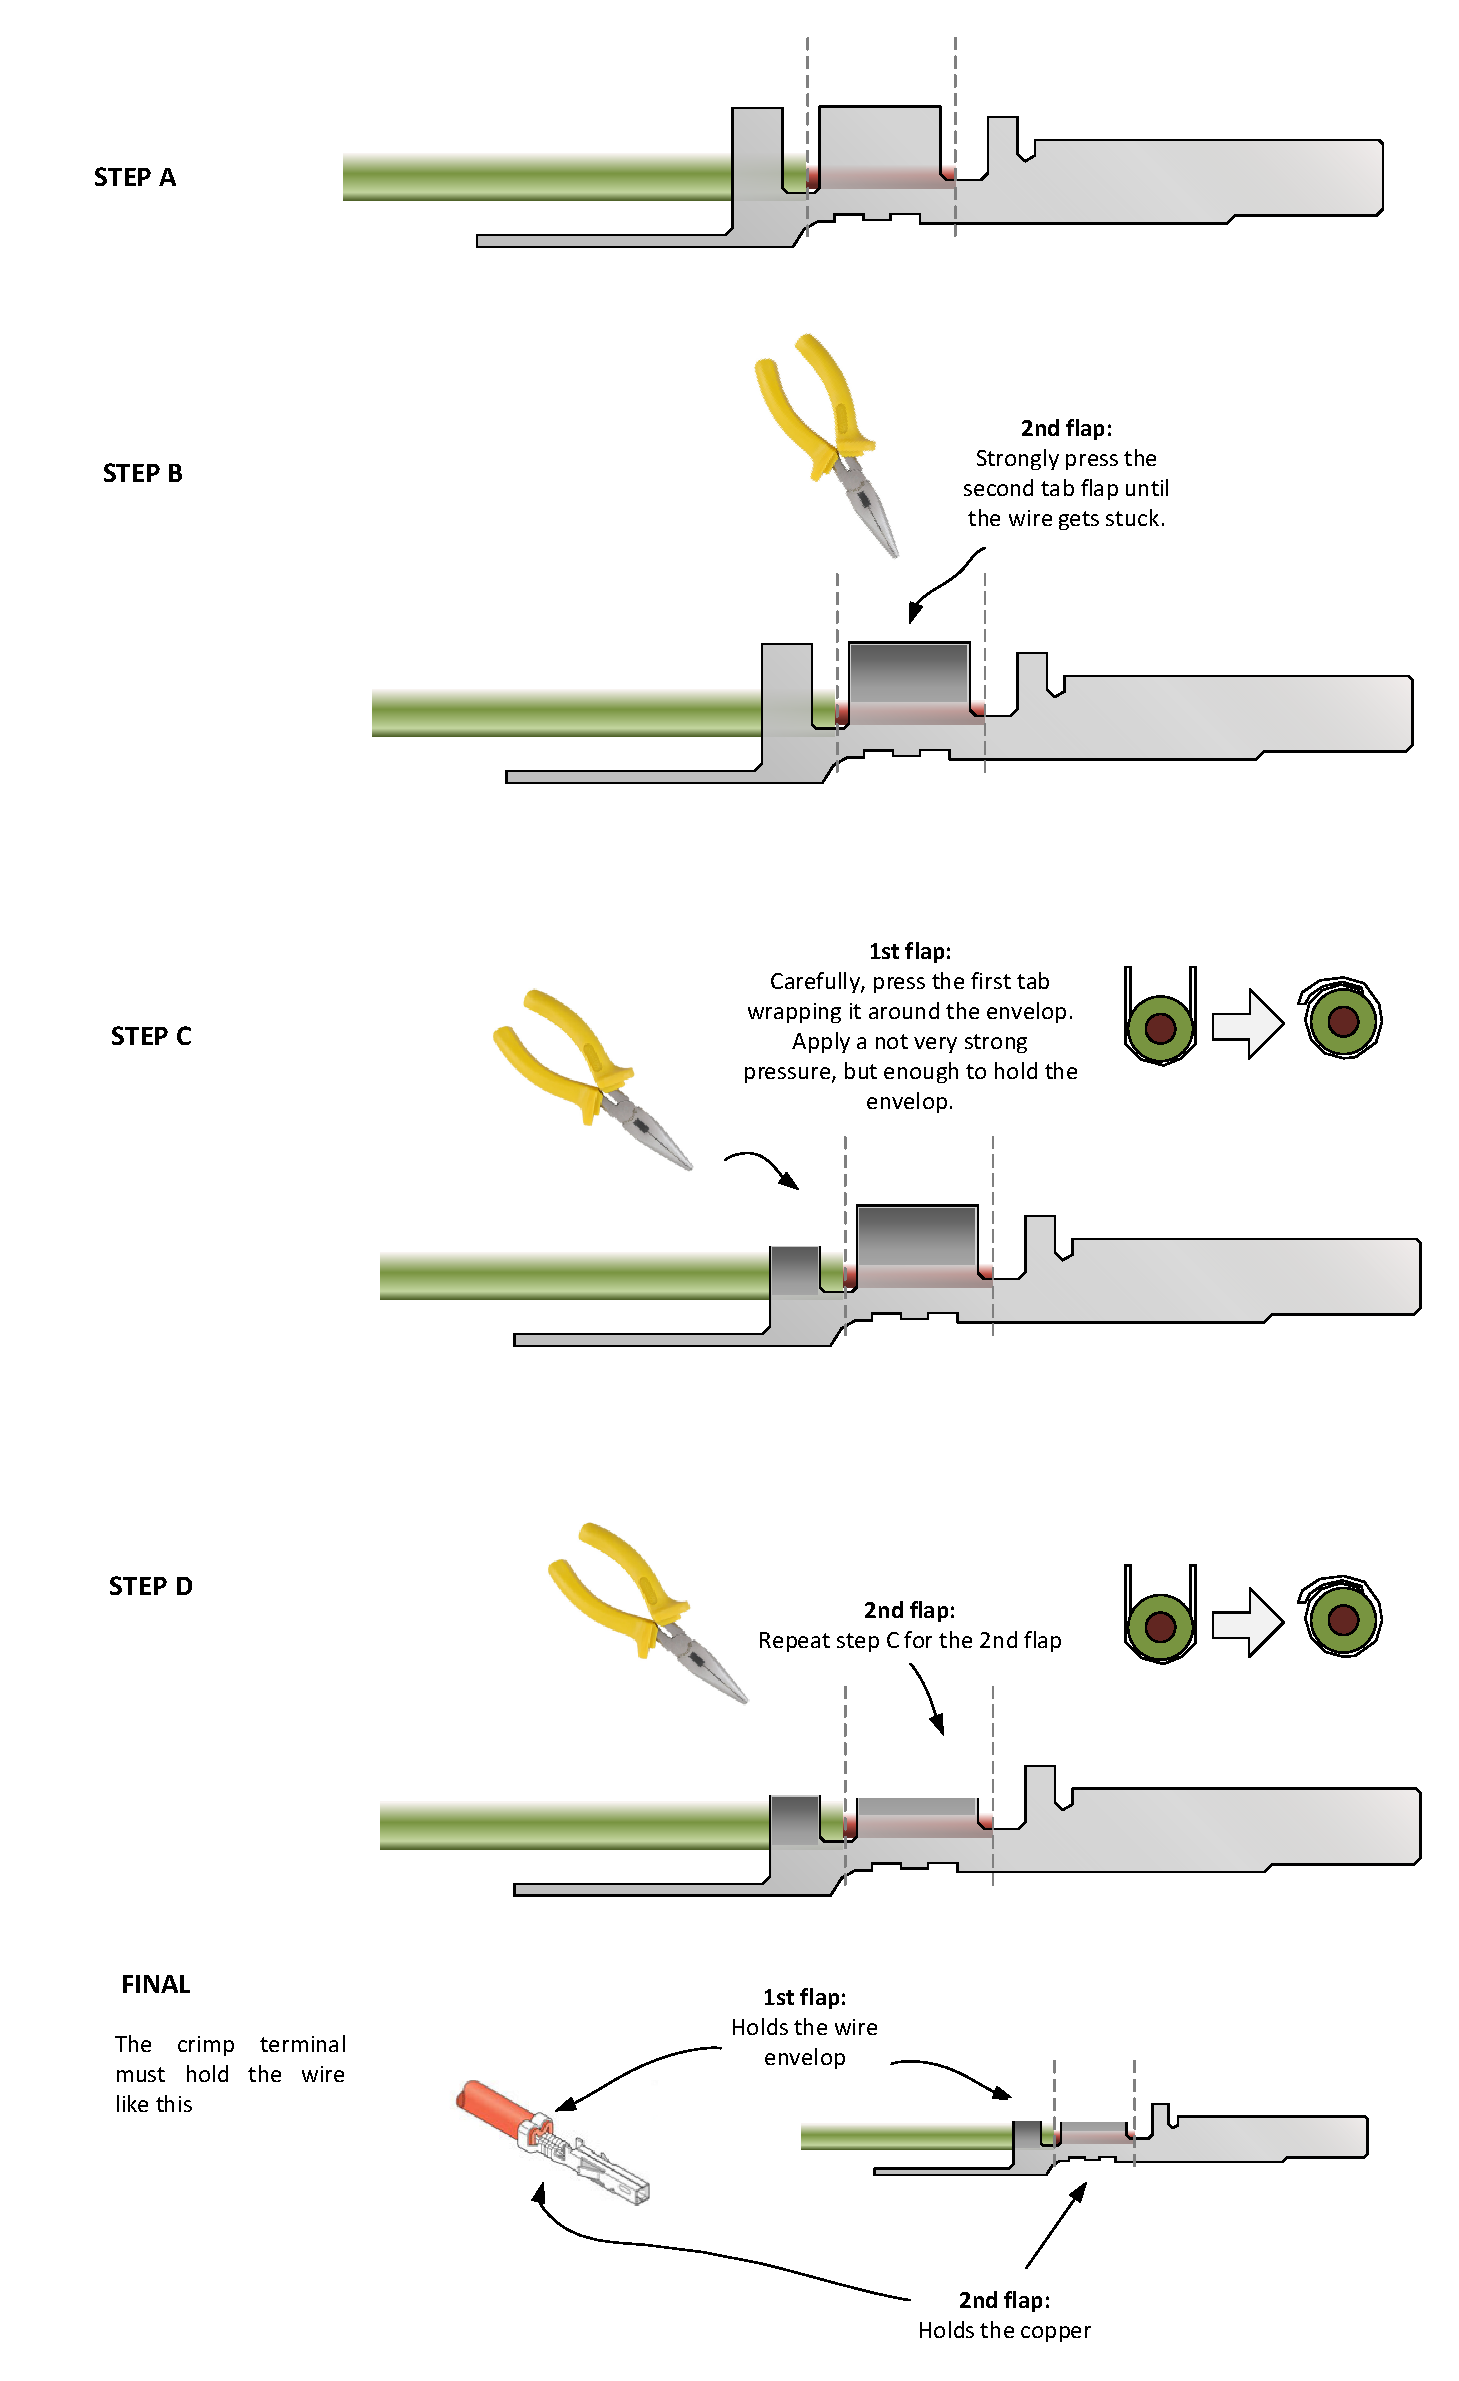
\includegraphics[angle=90,width=1\columnwidth]{figs/body03/FIGCRIMP6.pdf}\\
  \caption[Crimping Molex Mini-Fit \textregistered: procedures for manual crimping]{Crimping Molex Mini-Fit \textregistered: procedures for manual crimping}
  \label{FIG:CRIMP6}
\end{figure}
\begin{figure}
  \centering
  % Requires \usepackage{graphicx}
  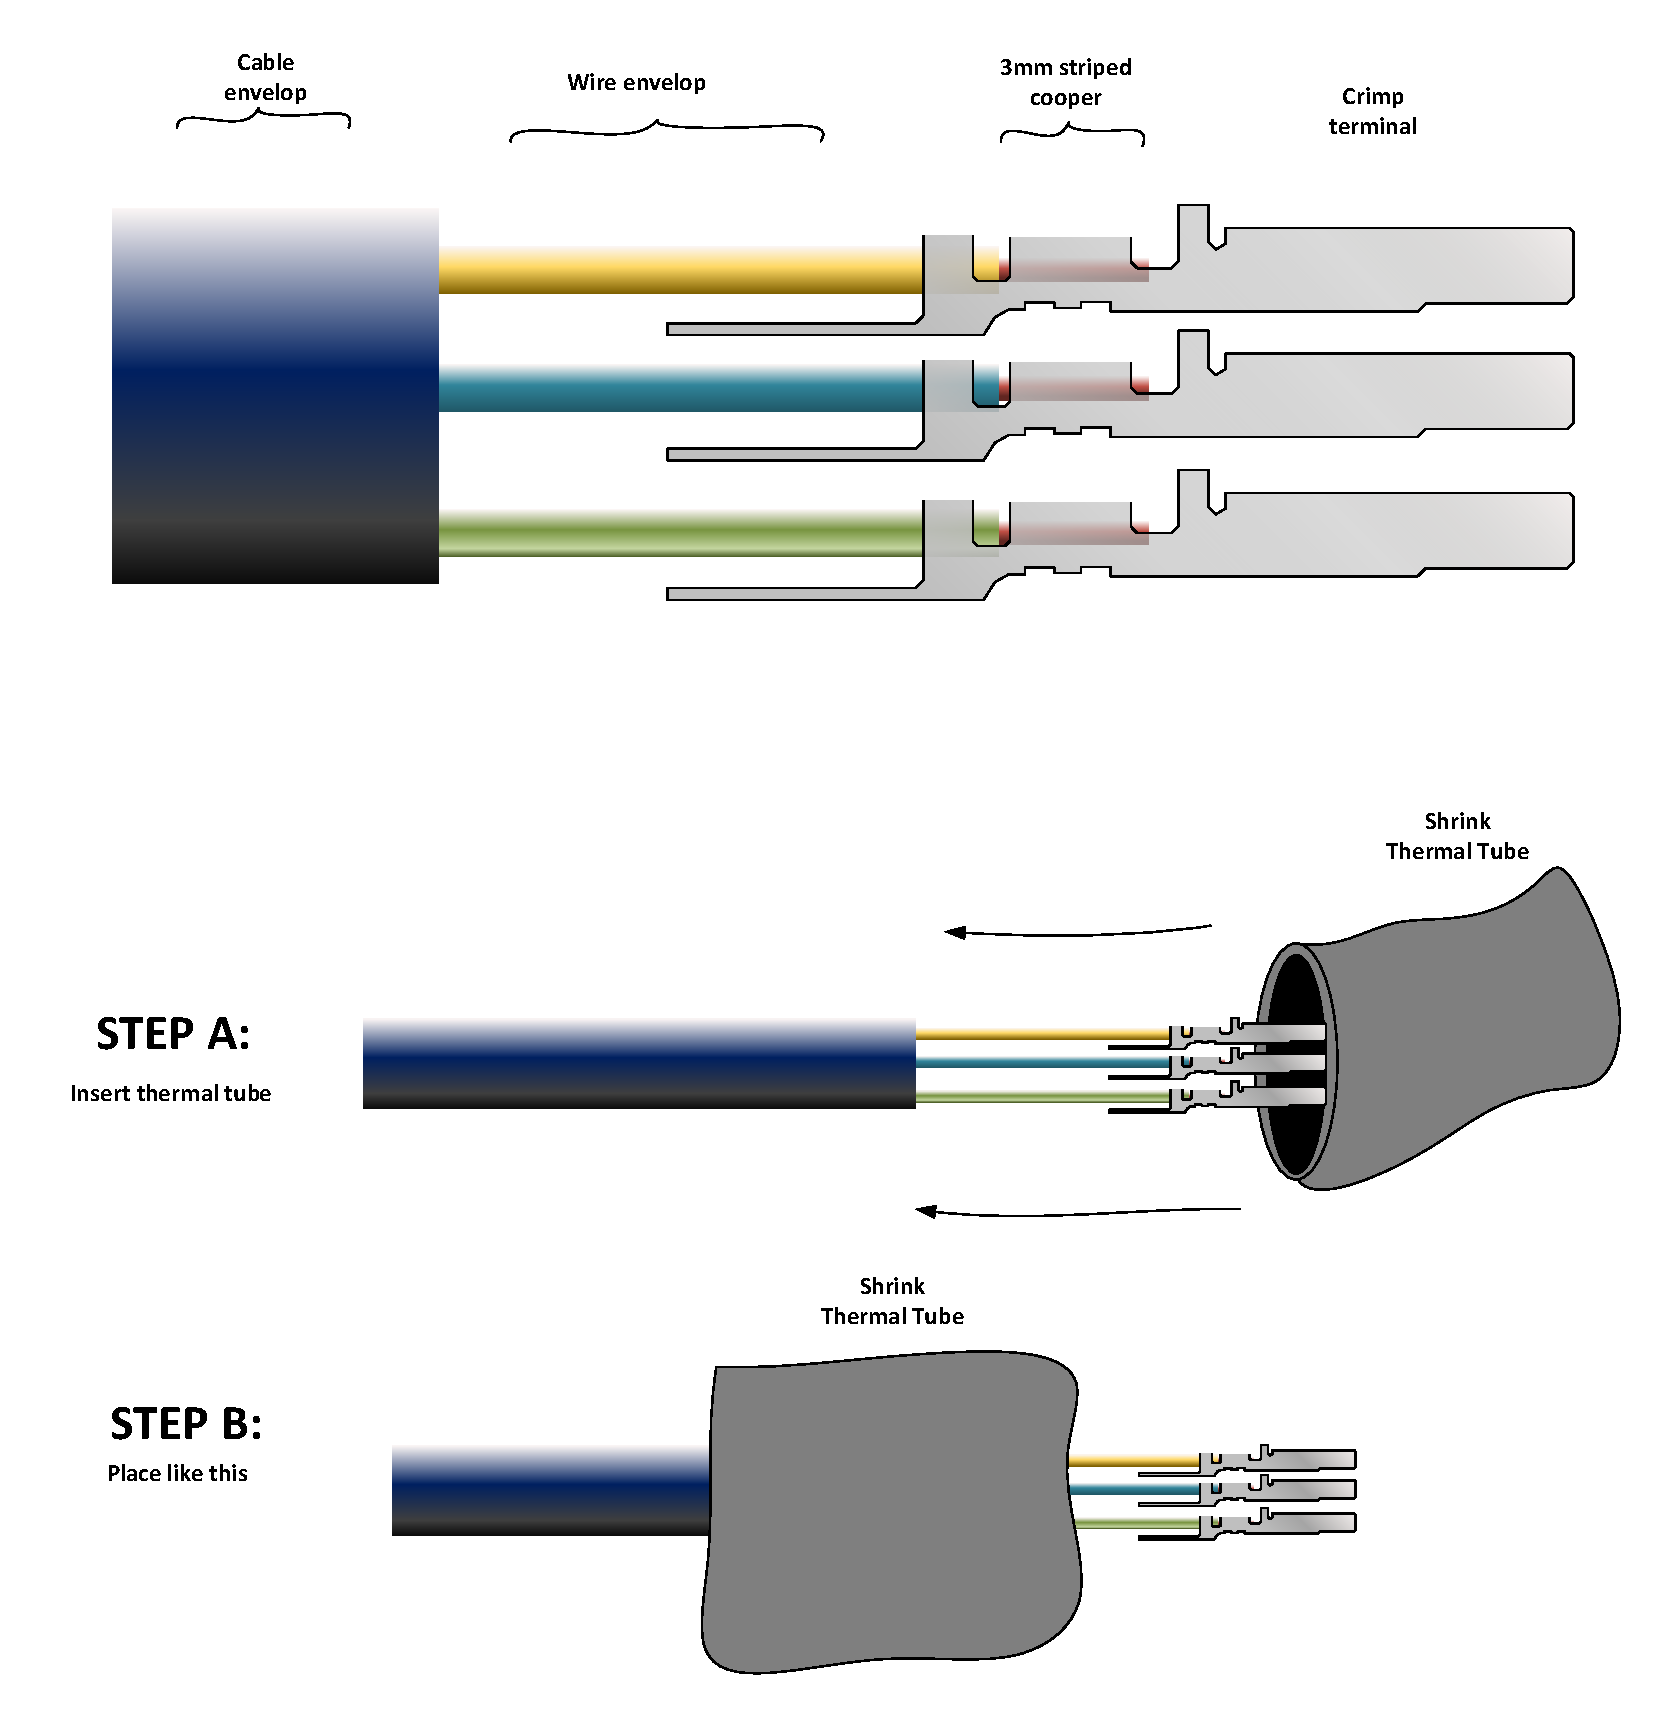
\includegraphics[angle=90,width=1\columnwidth]{figs/body03/FIGCRIMP7.pdf}\\
  \caption[Crimping Molex Mini-Fit \textregistered: applying the heat shrink tube]{Crimping Molex Mini-Fit \textregistered: applying the heat shrink tube}
  \label{FIG:CRIMP7}
\end{figure}
\begin{figure}
  \centering
  % Requires \usepackage{graphicx}
  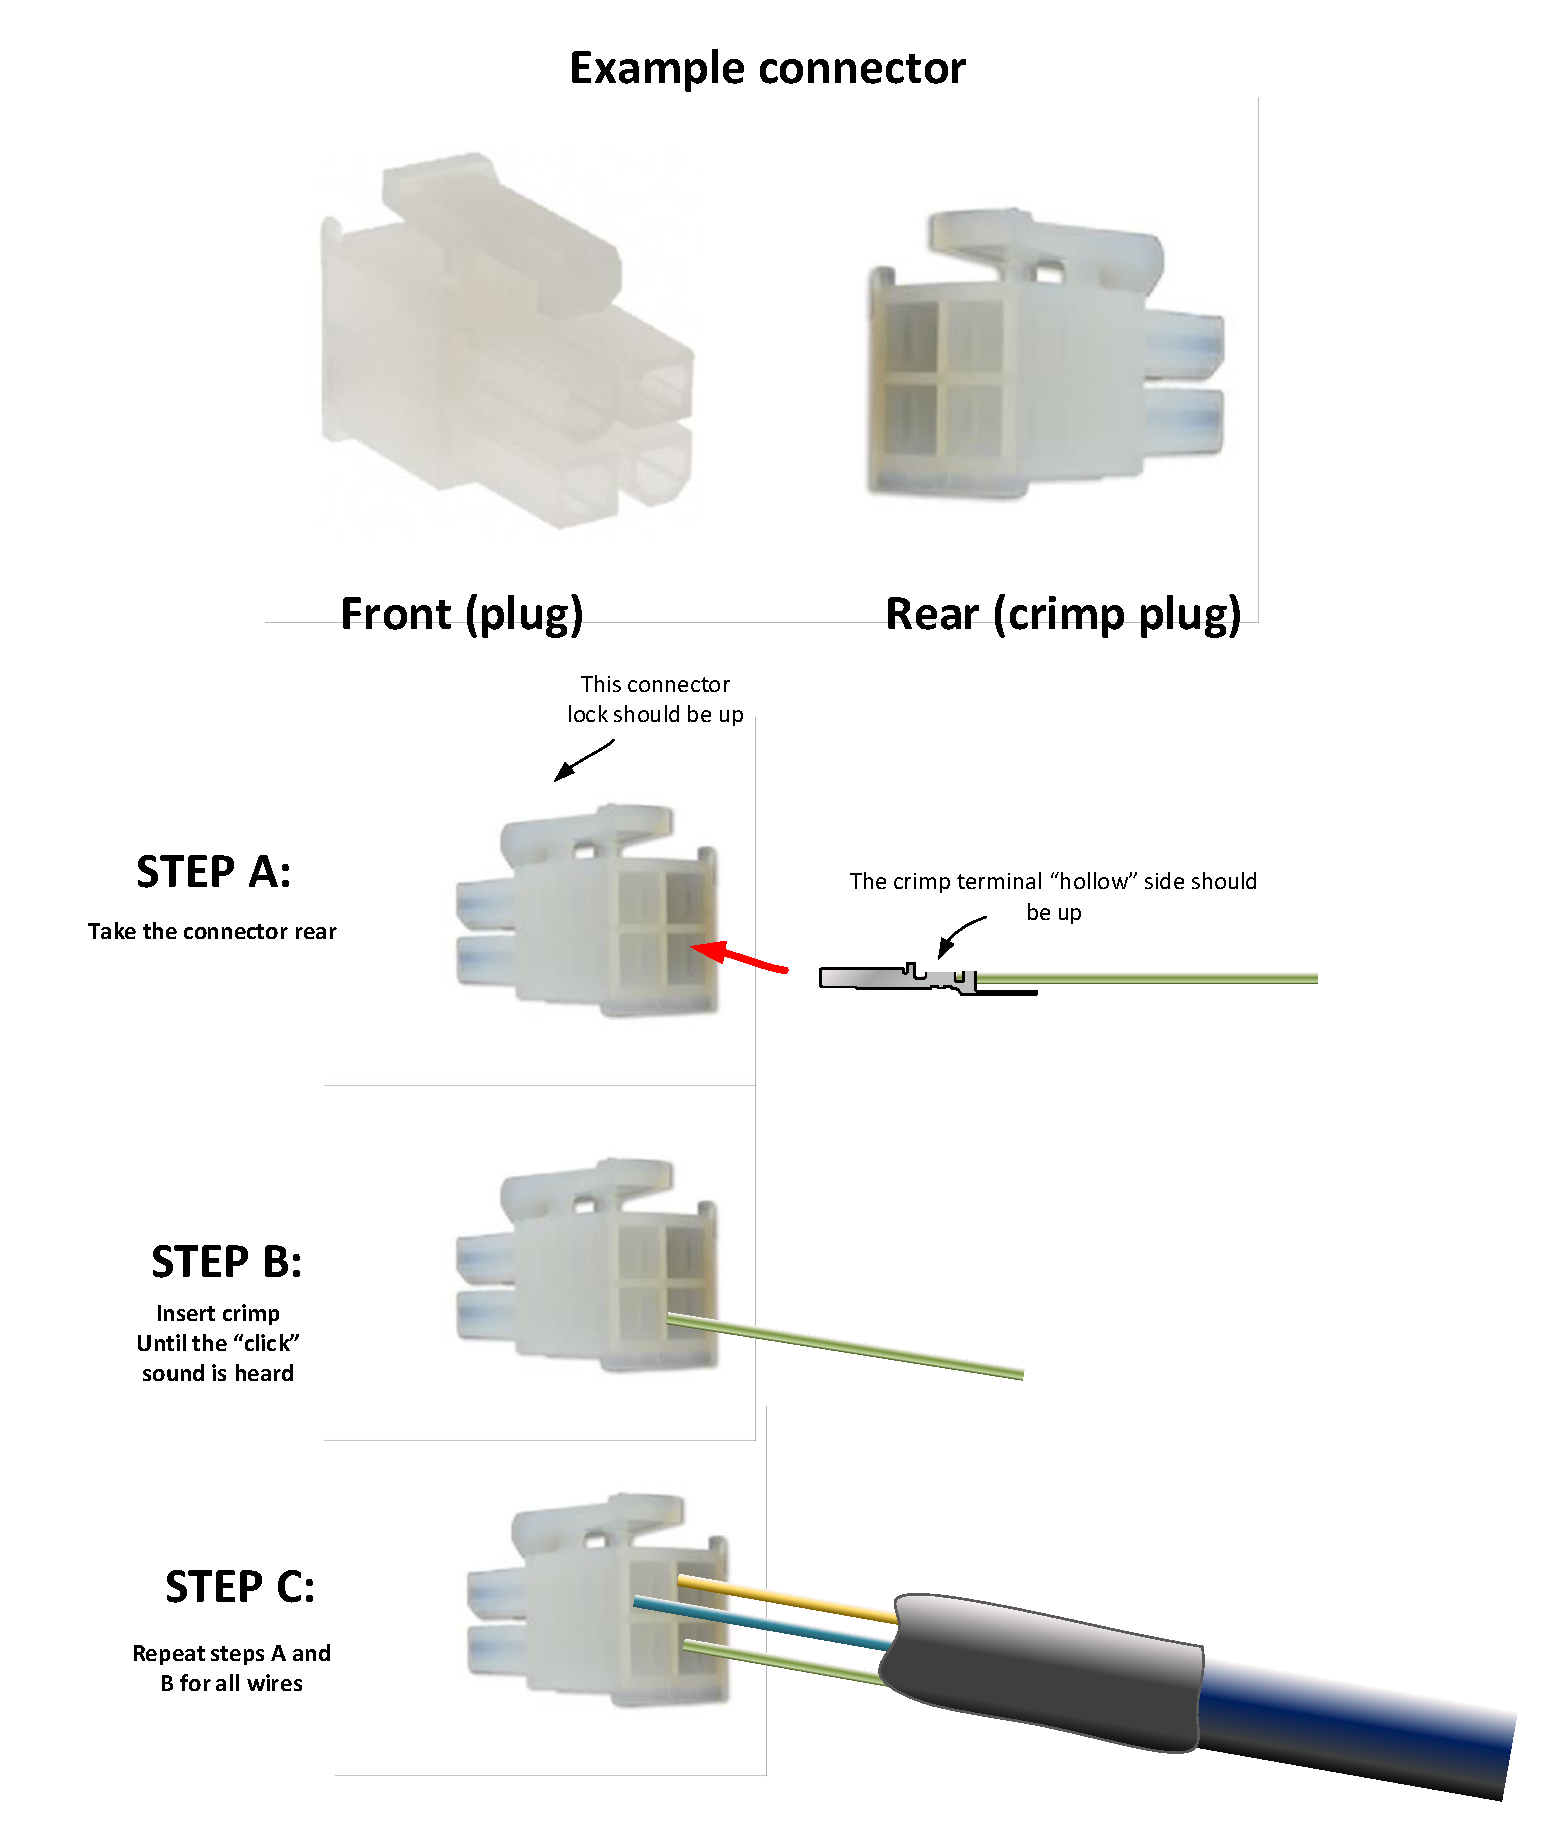
\includegraphics[angle=90,width=1\columnwidth]{figs/body03/FIGCRIMP8.pdf}\\
  \caption[Crimping Molex Mini-Fit \textregistered: inserting the crimp terminals into the connector holes]{Crimping Molex Mini-Fit \textregistered: inserting the crimp terminals into the connector holes}
  \label{FIG:CRIMP8}
\end{figure}
\subsection{Printed circuit boards (PCB) fabrication and assembly}
\section{System installation on site}
\section{System testing on site}
\section{System commissioning} 